
%% Beginning of file 'sample631.tex'
%%
%% Modified 2022 May  
%%
%% This is a sample manuscript marked up using the
%% AASTeX v6.31 LaTeX 2e macros.
%%
%% AASTeX is now based on Alexey Vikhlinin's emulateapj.cls 
%% (Copyright 2000-2015).  See the classfile for details.

%% AASTeX requires revtex4-1.cls and other external packages such as
%% latexsym, graphicx, amssymb, longtable, and epsf.  Note that as of 
%% Oct 2020, APS now uses revtex4.2e for its journals but remember that 
%% AASTeX v6+ still uses v4.1. All of these external packages should 
%% already be present in the modern TeX distributions but not always.
%% For example, revtex4.1 seems to be missing in the linux version of
%% TexLive 2020. One should be able to get all packages from www.ctan.org.
%% In particular, revtex v4.1 can be found at 
%% https://www.ctan.org/pkg/revtex4-1.

%% The first piece of markup in an AASTeX v6.x document is the \documentclass
%% command. LaTeX will ignore any data that comes before this command. The 
%% documentclass can take an optional argument to modify the output style.
%% The command below calls the preprint style which will produce a tightly 
%% typeset, one-column, single-spaced document.  It is the default and thus
%% does not need to be explicitly stated.
%%
%% using aastex version 6.3
\documentclass[twocolumn,twocolappendix]{aastex631}

%% The default is a single spaced, 10 point font, single spaced article.
%% There are 5 other style options available via an optional argument. They
%% can be invoked like this:
%%
%% \documentclass[arguments]{aastex631}
%% 
%% where the layout options are:
%%
%%  twocolumn   : two text columns, 10 point font, single spaced article.
%%                This is the most compact and represent the final published
%%                derived PDF copy of the accepted manuscript from the publisher
%%  manuscript  : one text column, 12 point font, double spaced article.
%%  preprint    : one text column, 12 point font, single spaced article.  
%%  preprint2   : two text columns, 12 point font, single spaced article.
%%  modern      : a stylish, single text column, 12 point font, article with
%% 		  wider left and right margins. This uses the Daniel
%% 		  Foreman-Mackey and David Hogg design.
%%  RNAAS       : Supresses an abstract. Originally for RNAAS manuscripts 
%%                but now that abstracts are required this is obsolete for
%%                AAS Journals. Authors might need it for other reasons. DO NOT
%%                use \begin{abstract} and \end{abstract} with this style.
%%
%% Note that you can submit to the AAS Journals in any of these 6 styles.
%%
%% There are other optional arguments one can invoke to allow other stylistic
%% actions. The available options are:
%%
%%   astrosymb    : Loads Astrosymb font and define \astrocommands. 
%%   tighten      : Makes baselineskip slightly smaller, only works with 
%%                  the twocolumn substyle.
%%   times        : uses times font instead of the default
%%   linenumbers  : turn on lineno package.
%%   trackchanges : required to see the revision mark up and print its output
%%   longauthor   : Do not use the more compressed footnote style (default) for 
%%                  the author/collaboration/affiliations. Instead print all
%%                  affiliation information after each name. Creates a much 
%%                  longer author list but may be desirable for short 
%%                  author papers.
%% twocolappendix : make 2 column appendix.
%%   anonymous    : Do not show the authors, affiliations and acknowledgments 
%%                  for dual anonymous review.
%%
%% these can be used in any combination, e.g.,
%%
%% \documentclass[twocolumn,linenumbers,trackchanges]{aastex631}
%%
%% AASTeX v6.* now includes \hyperref support. While we have built in specific
%% defaults into the classfile you can manually override them with the
%% \hypersetup command. For example,
%%
%% \hypersetup{linkcolor=red,citecolor=green,filecolor=cyan,urlcolor=magenta}
%%
%% will change the color of the internal links to red, the links to the
%% bibliography to green, the file links to cyan, and the external links to
%% magenta. Additional information on \hyperref options can be found here:
%% https://www.tug.org/applications/hyperref/manual.html#x1-40003
%%
%% Note that in v6.3 "bookmarks" has been changed to "true" in hyperref
%% to improve the accessibility of the compiled pdf file.
%%
%% If you want to create your own macros, you can do so
%% using \newcommand. Your macros should appear before
%% the \begin{document} command.
%%
\newcommand{\vdag}{(v)^\dagger}
\newcommand\aastex{AAS\TeX}
\newcommand\latex{La\TeX}

\usepackage{changepage} % for \begin{adjustwidth}{-Xcm}{} \end{adjustwidth}
%\usepackage{adjustbox}
\usepackage{rotating}


%\usepackage[colorlinks]{hyperref}
%\usepackage[draft]{hyperref}

%\usepackage{booktabs,caption}
\usepackage{tabularx} % for different number of columns in one Table
\usepackage{scrextend}
\let\orgautoref\autoref
\renewcommand{\autoref}
        {\def\equationautorefname{Eq.}%
         \def\figureautorefname{Fig.}%
         \def\sectionautorefname{Sect.}%
         \def\subsectionautorefname{Sect.}%
         \def\subsubsectionautorefname{Sect.}%
         \orgautoref}

\usepackage{xcolor}
\definecolor{dark-red}{rgb}{0.9,0.0,0.0}
\definecolor{dark-blue}{rgb}{0.15,0.15,0.9}
\definecolor{dark-green}{rgb}{0.15,0.8,0.15}
\definecolor{medium-blue}{rgb}{0,0,0.9}
\hypersetup{linkcolor={dark-blue},citecolor={dark-blue}, urlcolor={medium-blue}
}

\usepackage[flushleft]{threeparttable}

%% Reintroduced the \received and \accepted commands from AASTeX v5.2
%\received{March 1, 2021}
%\revised{April 1, 2021}
%\accepted{\today}

%% Command to document which AAS Journal the manuscript was submitted to.
%% Adds "Submitted to " the argument.
%\submitjournal{ApJL}

%% For manuscript that include authors in collaborations, AASTeX v6.31
%% builds on the \collaboration command to allow greater freedom to 
%% keep the traditional author+affiliation information but only show
%% subsets. The \collaboration command now must appear AFTER the group
%% of authors in the collaboration and it takes TWO arguments. The last
%% is still the collaboration identifier. The text given in this
%% argument is what will be shown in the manuscript. The first argument
%% is the number of author above the \collaboration command to show with
%% the collaboration text. If there are authors that are not part of any
%% collaboration the \nocollaboration command is used. This command takes
%% one argument which is also the number of authors above to show. A
%% dashed line is shown to indicate no collaboration. This example manuscript
%% shows how these commands work to display specific set of authors 
%% on the front page.
%%
%% For manuscript without any need to use \collaboration the 
%% \AuthorCollaborationLimit command from v6.2 can still be used to 
%% show a subset of authors.
%
%\AuthorCollaborationLimit=2
%
%% will only show Schwarz & Muench on the front page of the manuscript
%% (assuming the \collaboration and \nocollaboration commands are
%% commented out).
%%
%% Note that all of the author will be shown in the published article.
%% This feature is meant to be used prior to acceptance to make the
%% front end of a long author article more manageable. Please do not use
%% this functionality for manuscripts with less than 20 authors. Conversely,
%% please do use this when the number of authors exceeds 40.
%%
%% Use \allauthors at the manuscript end to show the full author list.
%% This command should only be used with \AuthorCollaborationLimit is used.

%% The following command can be used to set the latex table counters.  It
%% is needed in this document because it uses a mix of latex tabular and
%% AASTeX deluxetables.  In general it should not be needed.
%\setcounter{table}{1}

%%%%%%%%%%%%%%%%%%%%%%%%%%%%%%%%%%%%%%%%%%%%%%%%%%%%%%%%%%%%%%%%%%%%%%%%%%%%%%%%
%%
%% The following section outlines numerous optional output that
%% can be displayed in the front matter or as running meta-data.
%%
%% If you wish, you may supply running head information, although
%% this information may be modified by the editorial offices.
%\shorttitle{AASTeX v6.3.1 Sample article}
%\shortauthors{Schwarz et al.}
%%
%% You can add a light gray and diagonal water-mark to the first page 
%% with this command:
%% \watermark{text}
%% where "text", e.g., DRAFT, is the text to appear.  If the text is 
%% long you can control the water-mark size with:
%% \setwatermarkfontsize{dimension}
%% where dimension is any recognized LaTeX dimension, e.g., pt, in, etc.
%%
%%%%%%%%%%%%%%%%%%%%%%%%%%%%%%%%%%%%%%%%%%%%%%%%%%%%%%%%%%%%%%%%%%%%%%%%%%%%%%%%
%\graphicspath{{./}{figures/}}
%% This is the end of the preamble.  Indicate the beginning of the
%% manuscript itself with \begin{document}.

\begin{document}

\title{TOI-4504: Exceptionally
large Transit Timing Variations \\ induced by two resonant warm gas giants in a three planet system.}

%% LaTeX will automatically break titles if they run longer than
%% one line. However, you may use \\ to force a line break if
%% you desire. In v6.31 you can include a footnote in the title.

%% A significant change from earlier AASTEX versions is in the structure for 
%% calling author and affiliations. The change was necessary to implement 
%% auto-indexing of affiliations which prior was a manual process that could 
%% easily be tedious in large author manuscripts.
%%
%% The \author command is the same as before except it now takes an optional
%% argument which is the 16 digit ORCID. The syntax is:
%% \author[xxxx-xxxx-xxxx-xxxx]{Author Name}
%%
%% This will hyperlink the author name to the author's ORCID page. Note that
%% during compilation, LaTeX will do some limited checking of the format of
%% the ID to make sure it is valid. If the "orcid-ID.png" image file is 
%% present or in the LaTeX pathway, the OrcID icon will appear next to
%% the authors name.
%%
%% Use \affiliation for affiliation information. The old \affil is now aliased
%% to \affiliation. AASTeX v6.31 will automatically index these in the header.
%% When a duplicate is found its index will be the same as its previous entry.
%%
%% Note that \altaffilmark and \altaffiltext have been removed and thus 
%% can not be used to document secondary affiliations. If they are used latex
%% will issue a specific error message and quit. Please use multiple 
%% \affiliation calls for to document more than one affiliation.
%%
%% The new \altaffiliation can be used to indicate some secondary information
%% such as fellowships. This command produces a non-numeric footnote that is
%% set away from the numeric \affiliation footnotes.  NOTE that if an
%% \altaffiliation command is used it must come BEFORE the \affiliation call,
%% right after the \author command, in order to place the footnotes in
%% the proper location.
%%
%% Use \email to set provide email addresses. Each \email will appear on its
%% own line so you can put multiple email address in one \email call. A new
%% \correspondingauthor command is available in V6.31 to identify the
%% corresponding author of the manuscript. It is the author's responsibility
%% to make sure this name is also in the author list.
%%
%% While authors can be grouped inside the same \author and \affiliation
%% commands it is better to have a single author for each. This allows for
%% one to exploit all the new benefits and should make book-keeping easier.
%%
%% If done correctly the peer review system will be able to
%% automatically put the author and affiliation information from the manuscript
%% and save the corresponding author the trouble of entering it by hand.

\correspondingauthor{Michaela V\'{i}tkov\'{a}}
\email{vitkova@asu.cas.cz}

\author[0000-0002-2994-2929]{Michaela V\'{i}tkov\'{a}}
\affiliation{Astronomical Institute of the Czech Academy of Sciences, Fri\v{c}ova 298, CZ-25165 Ond\v{r}ejov, Czech Republic}
\affiliation{Department of Theoretical Physics and Astrophysics, Faculty of Science, Masaryk University, Kotl\'{a}\v{r}sk\'{a} 2, CZ-61137 Brno, Czech Republic}

\author[0000-0002-9158-7315]{Rafael Brahm} %rafael.brahm@uai.cl
\affiliation{Facultad de Ingeniera y Ciencias, Universidad Adolfo Ib\'{a}\~{n}ez, Av. Diagonal las Torres 2640, Pe\~{n}alol\'{e}n, Santiago, Chile}
\affiliation{Millennium Institute for Astrophysics, Chile}
\affiliation{Data Observatory Foundation, Chile}

\author[0000-0002-0236-775X]{Trifon Trifonov} %trifonov@mpia.de 
\affiliation{Max-Planck-Institut für Astronomie, Königstuhl 17, D-69117 Heidelberg, Germany}
\affiliation{Department of Astronomy, Sofia University ``St Kliment Ohridski'', 5 James Bourchier Blvd, BG-1164 Sofia, Bulgaria}
\affiliation{Landessternwarte, Zentrum f\"ur Astronomie der Universit\"at Heidelberg, K\"onigstuhl 12, D-69117 Heidelberg, Germany}

\author[0000-0002-1623-5352]{Petr Kab\'{a}th} %petr.kabath@asu.cas.cz 
\affiliation{Astronomical Institute of the Czech Academy of Sciences, Fri\v{c}ova 298, CZ-25165 Ond\v{r}ejov, Czech Republic}

\author[0000-0002-5389-3944]{Andr\'es Jord\'an} %andres.jordan@uai.cl
\affiliation{Facultad de Ingeniera y Ciencias, Universidad Adolfo Ib\'{a}\~{n}ez, Av. Diagonal las Torres 2640, Pe\~{n}alol\'{e}n, Santiago, Chile}
\affiliation{Millennium Institute for Astrophysics, Chile}
\affiliation{Data Observatory Foundation, Chile}

\author[0000-0002-1493-300X]{Thomas Henning} %henning@mpia.de (WINE)
\affiliation{Max-Planck-Institut für Astronomie, Königstuhl 17, D-69117 Heidelberg, Germany}

\author[0000-0002-5945-7975]{Melissa J. Hobson} %melihobson@gmail.com (WINE)
\affiliation{Observatoire de Genève, Département d'Astronomie, Université de Genève, Chemin Pegasi 51b, 1290 Versoix, Switzerland}

\author[0000-0003-3130-2768]{Jan Eberhardt} %eberhardt@mpia.de (WINE)
\affiliation{Max-Planck-Institut für Astronomie, Königstuhl 17, D-69117 Heidelberg, Germany}

\author[0009-0004-8891-4057]{Marcelo Tala Pinto} %marcelo.tala@edu.uai.cl (WINE)
\affiliation{Facultad de Ingeniera y Ciencias, Universidad Adolfo Ib\'{a}\~{n}ez, Av. Diagonal las Torres 2640, Pe\~{n}alol\'{e}n, Santiago, Chile}

\author[0000-0003-3047-6272]{Felipe I. Rojas} %firojas@uc.cl (WINE)
\affiliation{Instituto de Astrof\'isica, Facultad de F\'isica, Pontificia Universidad Cat\'olica de Chile, Chile}

\author[0000-0001-9513-1449]{Nestor Espinoza} %nespinoza@stsci.edu (WINE)
\affiliation{Space Telescope Science Institute, 3700 San Martin Drive, Baltimore, MD 21218, USA}

\author[0000-0001-8355-2107]{Martin Schlecker} %schlecker@arizona.edu (WINE)
\affiliation{Department of Astronomy/Steward Observatory, The University of Arizona, 933 North Cherry Avenue, Tucson, AZ 85721, USA}

\author{Mat\'{i}as I. Jones} %mjones@eso.org (WINE)
\affiliation{European Southern Observatory, Alonso de Córdova 3107, Vitacura, Casilla 19001, Santiago, Chile}

% \author[0000-0001-8128-3126]{Paula Sarkis} %paula.sarkis.90@gmail.com (WINE)
% \affiliation{Max-Planck-Institut für Astronomie, Königstuhl 17, D-69117 Heidelberg, Germany}

%\author{Leonardo Vanzi} %lvanzi@uc.cl (ANID-CAS joint project)
%\affiliation{Department of Electrical Engineering and Centre of Astro-Engineering, Pontificia Universidad Cat\'olica de Chile, Av. Vicu\~na Mackenna 4860, Santiago, Chile}

\author[0000-0002-7927-9555]{Maximiliano Moyano} %mmoyano@ucn.cl (ANID-CAS joint project)
\affiliation{Instituto de Astronom\'ia, Universidad Cat\'olica del Norte, Angamos 0610, 1270709, Antofagasta, Chile}

\author[0000-0003-4723-9660]{Susana Eyheramendy} %susana.eyheramendy@gmail.com (ANID-CAS joint project)
\affiliation{Facultad de Ingeniera y Ciencias, Universidad Adolfo Ib\'{a}\~{n}ez, Av. Diagonal las Torres 2640, Pe\~{n}alol\'{e}n, Santiago, Chile}
\affiliation{Millennium Institute for Astrophysics, Chile}
\affiliation{Data Observatory Foundation, Chile}

\author[0000-0002-0619-7639]{Carl Ziegler} %Carl.Ziegler@sfasu.edu (SOAR imaging)
\affiliation{Department of Physics, Engineering and Astronomy, Stephen F. Austin State University, 1936 North St, Nacogdoches, TX 75962, USA}

%\author{TESS contributing author} % we need to ask for this person to Avi Shporer (shporer@space.mit.edu) when the draft is more or less ready
%\affiliation{}
% below is the list of TESS architects. We need to cantact them to tess-architects@mit.edu and share the paper with them to confirm co-authorship.

\author[0000-0001-6513-1659]{Jack J. Lissauer}  %  jack.lissauer@nasa.gov
\affiliation{NASA Ames Research Center, Moffett Field, CA 94035, USA}

\author[0000-0001-7246-5438]{Andrew Vanderburg}  %andrew.vanderburg.astro@gmail.com
\affiliation{Department of Astronomy, University of Wisconsin-Madison, Madison, WI 53706, USA}

\author[0000-0001-6588-9574]{Karen A.\ Collins}  %karen.collins@cfa.harvard.edu 
\affiliation{Center for Astrophysics \textbar \ Harvard \& Smithsonian, 60 Garden Street, Cambridge, MA 02138, USA}

\author[0000-0002-5402-9613]{Bill Wohler} %bill.wohler@nasa.gov SPOC software/systems engineer
\affiliation{SETI Institute, Mountain View, CA 94043 USA/NASA Ames Research Center, Moffett Field, CA 94035 USA}

\author[0000-0002-3555-8464]{David Watanabe}
\affiliation{Planetary Discoveries, Valencia CA 91354, USA}

\author[0000-0003-2058-6662]{George R. Ricker}
\affiliation{Department of Physics and Kavli Institute for Astrophysics and Space Research, Massachusetts Institute of Technology, 77 Massachusetts Avenue, Cambridge, MA 02139, USA}

\author[0000-0001-6763-6562]{Roland Vanderspek}
\affiliation{Department of Physics and Kavli Institute for Astrophysics and Space Research, Massachusetts Institute of Technology, 77 Massachusetts Avenue, Cambridge, MA 02139, USA}

% \author[0000-0001-9911-7388]{David W. Latham}
% \affiliation{Center for Astrophysics \textbar \ Harvard \& Smithsonian, 60 Garden Street, Cambridge, MA 02138, USA}

\author[0000-0002-6892-6948]{Sara Seager}
\affiliation{Department of Physics and Kavli Institute for Astrophysics and Space Research, Massachusetts Institute of Technology, 77 Massachusetts Avenue, Cambridge, MA 02139, USA}
\affiliation{Department of Earth, Atmospheric and Planetary Sciences, Massachusetts Institute of Technology, 77 Massachusetts Avenue, Cambridge, MA 02139, USA}
\affiliation{Department of Aeronautics and Astronautics, Massachusetts Institute of Technology, 77 Massachusetts Avenue, Cambridge, MA 02139, USA}

\author[0000-0002-4265-047X]{Joshua N.\ Winn}
\affiliation{Department of Astrophysical Sciences, Princeton University, Princeton, NJ 08544, USA}

\author[0000-0002-4715-9460]{Jon M. Jenkins}
\affiliation{NASA Ames Research Center, Moffett Field, CA 94035, USA}

\author[0000-0002-7602-0046]{Marek Skarka} %\fnmsep%\thanks{The paper}
\affiliation{Astronomical Institute of the Czech Academy of Sciences, Fri\v{c}ova 298, CZ-25165 Ond\v{r}ejov, Czech Republic}
\affiliation{Department of Theoretical Physics and Astrophysics, Faculty of Science, Masaryk University, Kotl\'{a}\v{r}sk\'{a} 2, CZ-61137 Brno, Czech Republic}

%\collaboration{20}{(AAS Journals Data Editors)}


%% Note that the \and command from previous versions of AASTeX is now
%% depreciated in this version as it is no longer necessary. AASTeX 
%% automatically takes care of all commas and "and"s between authors names.

%% AASTeX 6.31 has the new \collaboration and \nocollaboration commands to
%% provide the collaboration status of a group of authors. These commands 
%% can be used either before or after the list of corresponding authors. The
%% argument for \collaboration is the collaboration identifier. Authors are
%% encouraged to surround collaboration identifiers with ()s. The 
%% \nocollaboration command takes no argument and exists to indicate that
%% the nearby authors are not part of surrounding collaborations.

%% Mark off the abstract in the ``abstract'' environment. 

% abstract has a 250 word limit
\begin{abstract}
We present a joint analysis of TTVs and Doppler data for the transiting exoplanet system TOI-4504. TOI-4504\,c is a warm Jupiter-mass planet that exhibits the largest known transit timing variations (TTVs), with a peak-to-node amplitude of $\sim$ 2\,days, the largest value ever observed, and a super-period of $\sim$ 930\,d. TOI-4504\,b and c were identified in public TESS data, while the TTVs observed in TOI-4504\,c, together with radial velocity (RV) data collected with FEROS, allowed us to uncover a third, non-transiting planet in this system, TOI-4504\,d. We were able to detect transits of TOI-4504\,b in the TESS data with a period of 2.4261$\pm 0.0001$\,days and derive a radius of 2.69$\pm 0.19$\,R$_{\oplus}$. The RV scatter of TOI-4504 was too large to constrain the mass of TOI-4504\,b, but the RV signals of TOI-4504\,c \& d were sufficiently large to measure their masses. The TTV+RV dynamical model we apply confirms TOI-4504\,c as a warm Jupiter planet with an osculating period of 82.54$\pm 0.02$\,d, mass of 3.77$\pm 0.18$\,M$_{\rm J}$ and a radius of 0.99$\pm 0.05$\,R$_{\rm J}$, while the non-transiting planet TOI-4504\,d, has an orbital period of 40.56$\pm 0.04$\,days and mass of 1.42$_{-0.06}^{+0.07}$\,M$_{\rm J}$. We present the discovery of a system with three exoplanets: a hot sub-Neptune and two warm Jupiter planets. The gas giant pair is stable and likely locked in a first-order 2:1 mean-motion resonance (MMR). The TOI-4504 system is an important addition to MMR pairs, whose increasing occurrence supports a smooth migration into a resonant configuration during the protoplanetary disk phase. 
\end{abstract}

%% Keywords should appear after the \end{abstract} command. 
%% The AAS Journals now uses Unified Astronomy Thesaurus concepts:
%% https://astrothesaurus.org
%% You will be asked to selected these concepts during the submission process
%% but this old "keyword" functionality is maintained in case authors want
%% to include these concepts in their preprints.
%\keywords{Classical Novae (251) --- Ultraviolet astronomy(1736) --- History of astronomy(1868) --- Interdisciplinary astronomy(804)}
\keywords{Exoplanet dynamics (490) --
Transit photometry (1709) --
Transit timing variation method (1710) --
Radial velocity (1332)
}
%planetary systems -- 
%   %optical: stars -- 
%   stars: late-type -- 
%   stars: low-mass -- 
%   planets and satellites}
%% From the front matter, we move on to the body of the paper.
%% Sections are demarcated by \section and \subsection, respectively.
%% Observe the use of the LaTeX \label
%% command after the \subsection to give a symbolic KEY to the
%% subsection for cross-referencing in a \ref command.
%% You can use LaTeX's \ref and \label commands to keep track of
%% cross-references to sections, equations, tables, and figures.
%% That way, if you change the order of any elements, LaTeX will
%% automatically renumber them.
%%
%% We recommend that authors also use the natbib \citep
%% and \citet commands to identify citations.  The citations are
%% tied to the reference list via symbolic KEYs. The KEY corresponds
%% to the KEY in the \bibitem in the reference list below. 

\section{Introduction} \label{sec:intro}

More than 5,000 transiting exoplanets have been identified. In a Keplerian system, transits occur at regular intervals. However, if additional planets are present in a system and their gravitational interactions are significant on observable timescales, then Transit Timing Variations \citep[TTVs,][]{TTV1,TTV2} are expected over the observed baseline. In particular, planets in or near low-order mean-motion resonances (MMRs) exhibit the largest TTV signals \citep{AGOL2005}. TTVs provide important constraints on the planetary masses and orbital parameters in the system and sometimes help uncover non-transiting planets. For instance, the first non-transiting planet fully characterized through TTVs was Kepler-46\,c \citep{KEPLER46}, which induced TTVs on the transiting planet Kepler-46\,b. Another example is Kepler-88\,b with a TTV amplitude of approximately 12 hours (peak-to-node), earning it the title ``the King of TTVs" \citep{KOI-142}. These TTVs revealed a pair of planets near the 2:1 MMRs. Another case of 2:1 resonance causing the peak-to-node TTVs of $\sim$ 1 day can be seen in Kepler-30\,b \citep{Kepler30a,Kepler30b}. Kepler-90\,g has a variation of 25.7 hours in the time lapsed between consecutive transits, but only a few transits have been observed, and the full amplitude of variation is not known \citep{Kepler90}.

Currently, we know of 30 planets discovered by TTVs\footnote{NASA Exoplanet Archive, Sept 3, 2024: \url{https://exoplanetarchive.ipac.caltech.edu}}, and more are being detected by NASA’s Transiting Exoplanet Survey Satellite \citep[TESS,][]{TESS}. TESS aims to detect transiting planets around relatively bright stars that are suitable for precise radial velocity (RV) measurements and, in rare cases, could help uncover non-transiting planets through TTVs. A combination of precise RV measurements and TTVs helps determine the planetary mass, radius, bulk density, and other important physical parameters.


\begin{table}[ht!]
\caption{Stellar parameters of TOI-4504.}
\centering
\label{star_params}
%\renewcommand{\arraystretch}{1} % Default value: 1
\begin{tabular}{ccc}
 % \\[-2ex]
 \hline 
  \hline
Parameter     & Value                   & Reference                        \\ \hline
Names         & TIC 349972412, TOI-4504 & TIC v8.2                             \\
%              & J07375217-6204416       & 2MASS                            \\
%              & 5289275864525400704     & Gaia DR3                         \\
RA (J2000)            & 07$^{\rm{h}}$ 37$^{\rm{m}}$ 52.1529498945$^{\rm{s}}$      & Gaia DR3                         \\
DEC (J2000)           & -62$^{\circ}$ 04$'$ 41.803583657$''$	      & Gaia DR3                         \\
%$\mu_{\alpha}$ [mas yr$^{-1}$]        & -8.582334835709297      & Gaia DR3                         \\
%$\mu_{\delta}$ [mas yr$^{-1}$]       & -8.26074211960362       & Gaia DR3                         \\
%$\pi$ [mas]           & 2.938011256174446       & Gaia DR3                         \\
T [mag]            & 12.5542                 & TIC v8.2                         \\
B [mag]            & 14.239                  & TIC v8.2                         \\
V [mag]            & 13.364                  & TIC v8.2                         \\
%J [mag]            & 11.714                  & 2MASS                            \\
%H [mag]            & 11.319                  & 2MASS                            \\
%K [mag]            & 11.236                  & 2MASS                            \\
distance [pc]     & 342.605 ${\pm}$ 1.707      & TIC v8.2                         \\
Spectral type & K1V                     & P\&M \\
T$_{\rm{eff}}$ [K]         & 5315 ${\pm}$ 60             & this work                         \\
$\log g$ [cm s$^{-2}$]        & 4.458$^{+0.021}_{-0.015}$       & this work                         \\
R$_{\star}$ [R$_{\odot}$]            & 0.92$^{+0.04}_{-0.04}$           & this work                         \\
M$_{\star}$ [M$_{\odot}$]             & 0.89$^{+0.06}_{-0.04}$         & this work                         \\
L$_{\star}$ [L$_{\odot}$]             & 0.62$^{+0.03}_{-0.03}$       & this work                         \\
$\rho_{\star}$ [kg m$^{-3}$]          & 1607$^{+93}_{-64}$        & this work         \\ 
\,[Fe/H] [dex]         & 0.16 ${\pm}$ 0.05     & this work                         \\
$v \cdot \sin i$ [km s$^{-1}$]             & 1.9 ${\pm}$ 0.5     & this work                         \\
Age [Gyr]             & 10.0$^{+2.9}_{-3.6}$    & this work                         \\
$\rm{A_V}$ [mag]             & 0.35$^{+0.07}_{-0.06}$    & this work                         \\
\hline
\hline
\end{tabular}
\tablecomments{P\&M: \cite{sp_type} \\ TIC v8.2: \cite{tic_1,tic_2} \\ Gaia DR3: \cite{gaia_a,gaia_b}} %2MASS: \cite{2MASS} \\ 
 \end{table}


 
\begin{figure}[ht!]
  \centering
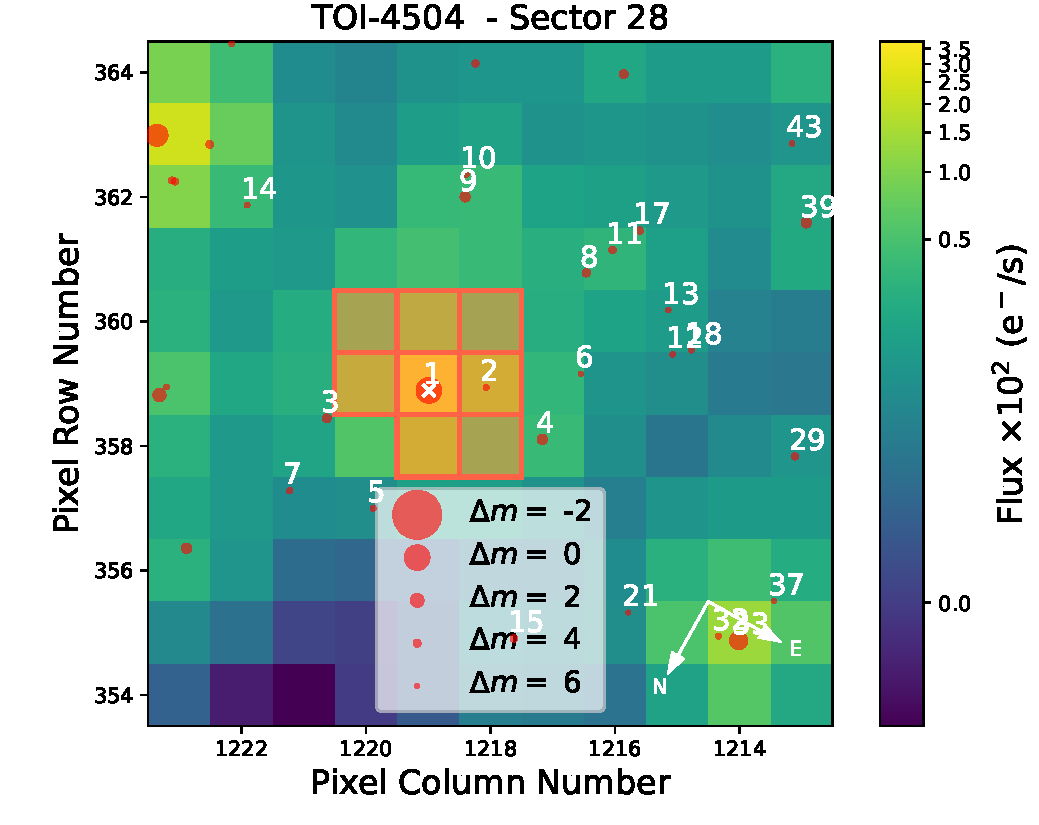
\includegraphics[width=0.48\textwidth]{TPF_Gaia_TIC349972412_S28.pdf}
  \caption{Target Pixel Files in Sector 28 for TOI-4504 obtained with {\textsc tpfplotter}. The shape of the aperture mask used to extract the photometry is marked with orange. Red dots indicate the sources of the Gaia DR3 catalogue in the field. TOI-4504 is marked with a white cross.}
  \label{TPF}
\end{figure}


In this work, we confirm the exoplanetary nature of the detected signal from TOI-4504. We firmly validate TOI-4504\,c, and report evidence for a non-transiting planet TOI-4504\,d that causes very strong TTVs of TOI-4504\,c. TOI-4504.01 (hereafter, TOI-4504\,c) was identified by The~Warm~gIaNts~with~tEss (WINE) collaboration, which is dedicated to the systematic characterization of TESS transiting warm giant planets \citep[see e.g.,][and references therein]{wine1,wine2,wine3,wine4,wine5,Bozhilov2023,TOI-199,jones2024}. The signature was referred to the TESS Science Office at MIT as a CTOI in May 2020, and the Quick Look Pipeline \citep[QLP,][]{QLPa,QLPb} was run to assess the candidate, identifying a period of P = 81.966 days. The TESS Science Processing Operations Center \citep[SPOC,][]{SPOC} independently detected transits of TOI-4504\,c in Sector 34 and several subsequent single- and multi-sector searches, using a noise-compensating matched filter \citep{Jenkins2002,Jenkins2020}, and an initial limb-darkened transit model was fit \citep{Li2019} and a suite of diagnostic tests were conducted to help make or break the planetary interpretation \citep{Twicken2018}. The shallower signal designated as TOI-4504.02 (hereafter TOI-4504\,b) was detected by the TESS Science Processing Operation Center \citep[SPOC,][]{SPOC} at NASA Ames Research Center with P = 2.4261 days in a search of sectors 27-36. Both TOI-4504\,b and c were alerted to the community by the TSO on 21 October 2021.

%Later, in October 2021, the TESS Science Office listed TOI-4504 in the Exo-FOP-TESS archive\footnote{\url{https://exofop.ipac.caltech.edu/tess/target.php?id=349972412}} to have two transiting exoplanet candidates. The deeper signal, TOI-4504.01 (hereafter, TOI-4504\,c), was detected by the MIT Quick Look Pipeline \citep[QLP,][]{QLPa,QLPb} with period $P=81.966$\,d, whereas the shallower signal designated as TOI-4504.02 (hereafter, TOI-4504\,b) was detected by the TESS Science Processing Operation Center \citep[SPOC,][]{SPOC} at NASA Ames Research Center with $P=2.4261$\,d. 

% ----------- SOAR data ------------
\begin{figure}[ht!]
  \centering
  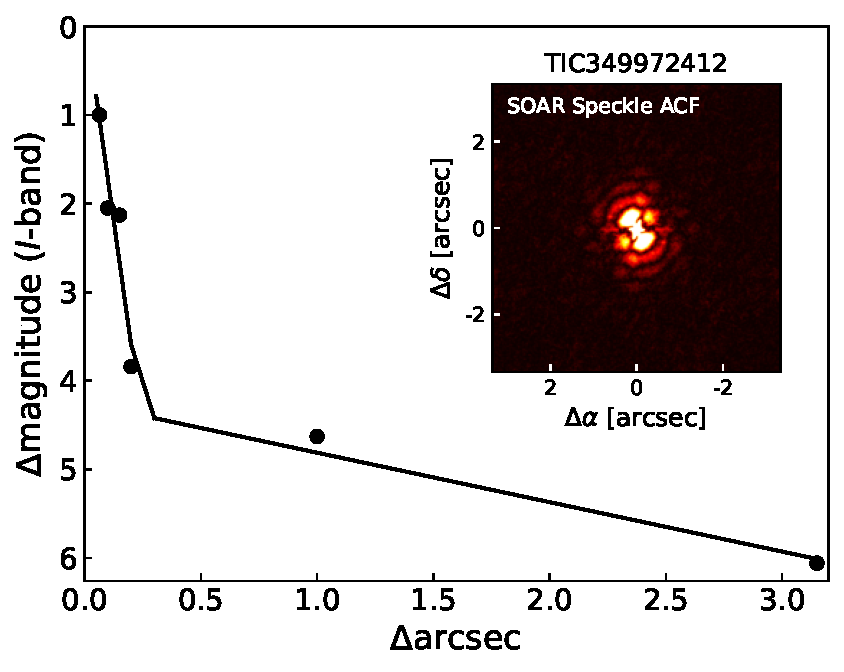
\includegraphics[width=0.9\linewidth]{TIC349972412I-cz20220415-2.pdf}
  \caption{High-resolution imaging from SOAR for TOI-4504. The inside image shows a speckle auto-correlation function. The 5$\sigma$ contrast curve is shown as the black points with the linear fit as the black solid line.}
  \label{Imaging}
\end{figure}


In this work, we report evidence for a non-transiting planet TOI-4504\,d that causes very strong TTVs of TOI-4504\,c. The induced TTVs on TOI-4504\,c have a semi-amplitude of a little less than 2 days (peak-to-peak of 4 days), making TOI-4504\,c a new record-holder for TTV signal amplitude.
Given the strong sinusoidal TTV signal we detect, near a low-order period ratio commensurability with the transiting planet is suspected. In such cases, the TTV periodic signal can be approximated by the so-called ``super-period":

\begin{equation}
{P}_{\mathrm{TTV}}={\left|\frac{j-1}{{P}_{\mathrm{in}}}-\frac{j}{{P}_{\mathrm{out}}}\right|}^{-1}.
\end{equation}

\noindent
where $j$ = $P_{\mathrm{out}}$/$P_{\mathrm{in}}$ represents the close commensurability between the inner and the outer planets. The observed super-period of TOI-4504 is $\sim$ 930\,d. Our fitting analysis of the observed data indicates that TOI-4504\,d is an inner Jovian-mass planet with a period of about 41 days, placing it in a 2:1 period-ratio commensurability with the transiting exoplanet TOI-4504\,c.



This paper is organized as follows: In \autoref{sec:observ}, we introduce the photometric and spectroscopic data collected for TOI-4504. In \autoref{sec3}, we present the stellar parameters 
of TOI-4504. In \autoref{sec4}, we introduce our orbital analysis and results. Finally, in \autoref{sec5}, we present a summary and our conclusions.

  


\section{Observations} 
\label{sec:observ}

\subsection{TESS photometry}
\label{sec:photo}
TOI-4504 was observed with a 30-minute cadence during the first year of the TESS primary mission in sectors 1-13. In the third and fifth years (sectors 27-38, 61-65, and 67-69), it was observed with a 120-second cadence. The image data were reduced and analyzed by the Science Processing Operations Center at NASA Ames Research Center.

We retrieved the 30-minute data using the {\textsc tesseract} pipeline\,\footnote{Available at \url{https://github.com/astrofelipe/tesseract}}(Rojas et al. in prep.). This pipeline extracts light curves from Full Frame Images (FFIs) using {\textsc TESSCut} \citep{tesscut} and {\textsc Lightkurve} \citep{lightkurve} packages. The download of the data with a 120\,s cadence was done with {\textsc Lightkurve}. Transits of TOI-4504\,c occur in sectors 3, 6, 9, 12, 28, 31, 34, 37, 61, 64 and 67. We used the Presearch Data Conditioning SAP flux (PDCSAP, \citealt{pdcsap1,pdcsap2,pdcsap3}) in all sectors where it is available. PDCSAP light curves are corrected for systematic trends. The transit present in sector 61 is cut off by a quality check in PDCSAP. This transit can be seen in Simple Aperture Photometry (SAP) data but is contaminated by background noise. It was possible to use data from this sector for measuring TOI-4504\,c transit time, but we did not use these data to fit the planet parameters. Analysis of TOI-4504\,c is described in more detail in \autoref{sec:4504c}.

For the TOI-4504\,b analysis, we used 120\,s cadence data available in sectors 27-38, 61-65, and 67-69 and used PDCSAP light curves. Analysis of TOI-4504\,c is described in \autoref{sec:4504b}. 


\subsection{Spectroscopic data}
\label{sec:spec}
Follow-up observations of TOI-4504 were performed with the FEROS spectrograph \citep{feros} mounted at the MPG 2.2m telescope at La Silla Observatory. TOI-4504 was observed between March 2020 and May 2024 in order to validate the transiting companions and constrain their masses. We obtained 39 spectra with exposure times of 1500 s and 1800 s and an average signal-to-noise ratio of 40. We used the {\textsc ceres} pipeline \citep{ceres} to process the data. From this pipeline, we obtained RV and stellar activity indicator such as CCF bisector spans (BIS, e.g., \cite{bis}), $\rm{H}_{\alpha}$ \citep{haplha}, $\log(R'_{HK})$ \citep{log,log2}, Na II, and He I \citep{he}.
Our extracted RVs and activity indices for TOI-4504 are listed in \autoref{RV_feros}. 


\subsection{Inspection of nearby sources}
\label{sec:contaminant}
For inspection of Target Pixel Files (TPF), we used {\textsc tpfplotter} \citep{tpfplotter}. It compares the {\it Gaia} DR3 catalogue with TESS TPF and allows us to see possible contamination in the field. In \autoref{TPF}, a TPF image of sector 28 is shown. In almost all sectors, a star with {\it Gaia} ID 5289275864525442048 (TIC 349972416, $G=18.48$\,mag, star '2' in \autoref{TPF}) is in the aperture mask. It is 5.4 magnitudes fainter than our object, and the distance between our target and TIC 349972416 is 19.37\,$''$. Among the multiple sector data, there are two additional sources, '3' and '4', which are often close or in the aperture; however, if the transit events were on the possible contaminator stars, the transit depth would vary substantially in the observed sectors, which were not observed. Our RVs show that the transits likely originate from the target star and not from this companion (\autoref{sec:spec}).
%The value of the contamination ratio (CR) is 2,79\,\% and therefore, we concluded that the transit signals originate from TOI-4504 and not from nearby stars.

To reject the contamination by sources closer than $\sim$2 \,$''$ from the target star, we used the 4.1-m SOAR telescope \citep{SOAR} within the SOAR TESS survey \citep{SOAR_TESS} to obtain speckle imaging. The images were obtained on 15 April 2022 with a Cousins I filter and a resolution of 36 mas, and they did not reveal any nearby sources. In \autoref{Imaging}, the speckle auto-correlation function and the contrast curve are shown. It reaches a contrast of $\Delta$mag = 4.5 at 0.5\,arcsec, and an estimated point spread function (PSF) is 0.064\,arcsec. There is no apparent nearby contaminant within 3\,arcsec from the target (\autoref{Imaging}).
Furthermore, the Gaia Renormalised Unit Weight Error (RUWE) value 1.12 of our object also indicates that the single-star model fits the astrometric observations well.
Additionally, the SPOC difference image centroid test was able to localize the host star to within 0.33 $\pm$ 2.7\,arcsec of the transit source location (averaged over the different TCEs in the S27-69 search) for TOI-4504\,c, and to 1.8 $\pm$ 3.1\,arcsec of the transit source location for TOI-4504\,b (based on the S27-69 search).% for TOI-4504\,c and for TOI-4504\,b.

%-------------------------------------------------------------------------------------------
\subsection{Follow-up photometry}
Several follow-up photometric observations of TOI-4504\,c were conducted and are available in Exo-FOP. Eight observations were scheduled to record the transit of TOI-4504\,c, assuming a constant period, but all resulted in non-detections. The non-detections, potentially due to the large TTVs, make it harder to predict the next transit. We include our predictions for upcoming transits in \autoref{sec:prediction}.
There are two observations of TOI-4504\,b, but since this exoplanet does not directly contribute to detected TTVs aimed to be studied in this work, this observation was excluded from the modeling scheme.




\begin{table}[ht!]
\caption{Priors and posteriors for TOI-4504\,b parameters derived with {\textsc juliet}.}
\centering
\label{02_transit_fit}
\begin{tabular}{ccc}
 \hline 
  \hline
Parameter       & Prior                         & Posterior                           \\ \hline
$P$ [days]               & $\mathcal{N}$ (2.4,0.5)       & $2.42614^{+0.00014}_{-0.00013}$           \\
$t_0$ [BJD]               & $\mathcal{N}$ (2459038.46,0.2)       & $2459038.458^{+0.022}_{-0.021}$           \\

$b$               & $\mathcal{U}$ (0.0,1.0)       & $0.396^{+0.134}_{-0.197}$           \\
$R_p/R_{\star}$               & $\mathcal{U}$ (0.0,1.0)       & $0.0268^{+0.0019}_{-0.0019}$           \\
$q_1$        & $\mathcal{U}$ (0.0,1.0)       & $0.527^{+0.320}_{-0.308}$           \\
$q_2$        & $\mathcal{U}$ (0.0,1.0)       & $0.496^{+0.323}_{-0.316}$           \\
$e$               & fixed 0.0                     & --                                  \\
$\omega$ [$^\circ$]           & fixed 90.0                    & --                                  \\
$\rho_{\star}$ [kg cm$^{-3}$]             & $\mathcal{N}$ (1600,100)      & $1601^{+100}_{-97}$                \\
$m_{\rm dilution}$ & fixed, 1.0                    & --                                  \\
$m_{\rm flux}$     & $\mathcal{N}$ (0.0,0.1)       & $-0.000046^{+0.000014}_{-0.000014}$ \\
$\sigma_w$ [ppm]  & $\mathcal{J}$ (0.1,1000.0)    & $2.16^{+17.11}_{-1.90}$                   \\
$a$ [au]               & --                            & $0.03392 \pm 0.00068$                  \\
$R_p$ [$R_{\oplus}$]   & --                            & $2.691 \pm 0.191$                  \\
$i$ [$^\circ$]   & --                            & $87.4^{+0.9}_{-1.3}$                  \\
\hline
\hline
\end{tabular}
\tablecomments{$a$ is calculated using Kepler's third law and derived period $P$}
\end{table}

We conclude that TOI-4504 is a metal-rich ([Fe/H]$ = 0.16\pm0.05$\,dex) main sequence star ($M_{\star} = 0.89^{+0.06}_{-0.04}$\,M$_{\odot}$, $R_{\star} = 0.92^{+0.04}_{-0.04}$\,R$_{\odot}$), just on the boundary between a G- and K-type star ($T_{\rm{eff}} = 5315 \pm 60$\,K). 




\section{Stellar parameters of TOI-4504}
\label{sec3}

We followed the two-step iterative procedure presented in \citet{wine1} to obtain the stellar parameters of the host star. We start from the co-added FEROS spectra to obtain the stellar atmospheric parameters ($T_{\rm{eff}}$, $\log g$, [Fe/H], $v \sin i$) using the \textsc{zaspe} package \citep{zaspe}.%, which compares the observed spectra against a grid of synthetic models, focusing on the regions of the spectrum that are most sensitive to changes in the parameters. 
We perform a spectral energy distribution (SED) fit to estimate the stellar physical parameters, using the publicly available broad-band photometry as data and the PARSEC isochrones as a model. This step involved the use of the GAIA DR3 \citep{gaia_b} parallax to convert the observed apparent magnitudes to absolute magnitudes and adopt a simple interstellar extinction rule \citep{cardelli:1989}. 

We also fix the metallicity to the one derived with \textsc{zaspe} and use the \textsc{zaspe} value for the $T_{\rm{eff}}$ as a prior. This step produces a more precise value for the stellar $\log g$, which is used as input in a new run of \textsc{zaspe}. We continue with the iterations until reaching convergence of the $T_{\rm{eff}}$ and [Fe/H] in two subsequent \textsc{zaspe} runs.
Stellar parameters from our analysis are listed in \autoref{star_params}.
The uncertainties in the stellar parameters obtained with our procedure do not include possible systematic differences with respect to other stellar models; because of this, we inflate the uncertainties as suggested in \cite{Tayar_2022}.


%-------------------------------------------------------------
\section{Analysis and Results}
\label{sec4}

% Did we use TLS to identify TOI-4504\,c: Ask Rafa.


\begin{figure}[ht]
  \centering
  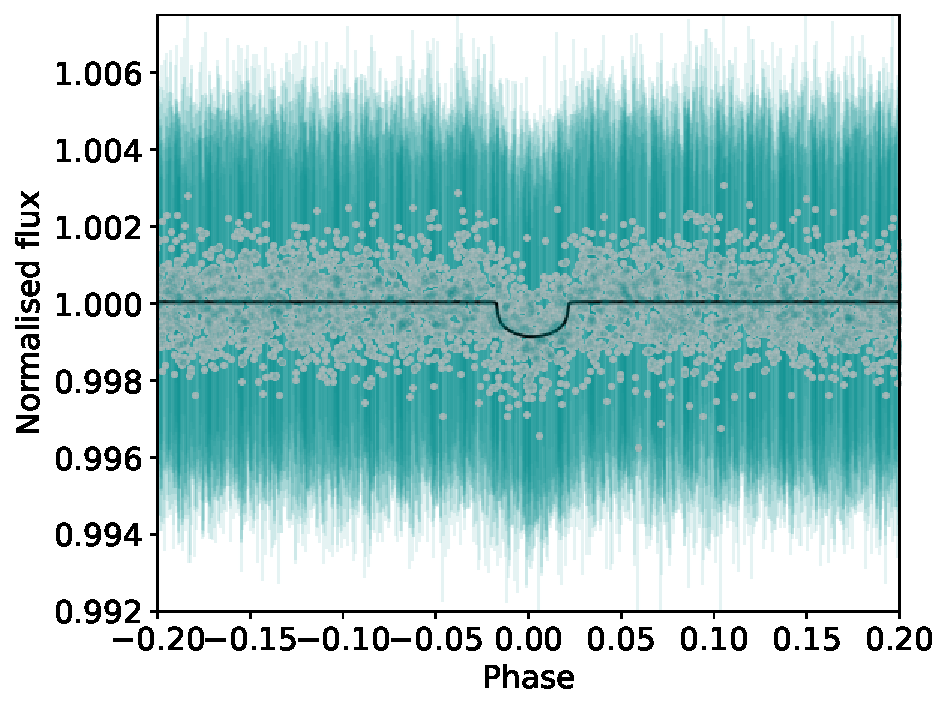
\includegraphics[width=1\linewidth]{02_phased.pdf}
  \caption{Phase plot for TOI-4504\,b transit. Light curve was binned into one-hour bins.}
  \label{02_transit_fit_fig}
\end{figure}


\subsection{Transit analysis and TTV extraction}
\label{sec:ttv}

For the transit fitting, we used the python package {\textsc juliet} \citep{juliet}, which employs transit light-curve models from the {\textsc batman} package \citep{batman}. Transit analysis of each planet was treated individually.

\subsubsection{TOI-4504\,b}
\label{sec:4504b}
For the transit analysis of TOI-4504\,b, we used 2-min PDCSAP data. Before the analysis, we deleted transits of TOI-4504\,c from the time series. We used broad uninformative priors (see \autoref{02_transit_fit}). The final values of the fit are also listed in \autoref{02_transit_fit}. 


\autoref{02_transit_fit_fig} shows binned data that are phase-folded with the orbital period of 2.42614\,days together with the fit of the transit. We detected a planet with a transit depth of $\Delta F=718$\,ppm. %which translates into a planetary radius of $R_{\rm p}=2.689(191)$\,R$_{\oplus}$. 
Our RV data were insufficient to confirm this planet and estimate its mass (see \autoref{feros_anaysis}). However, the radius of $R_{\rm p}=2.691 \pm 0.191$\,R$_{\oplus}$ and mass of $10.4 \pm 0.9$\,M$_{\oplus}$ calculated from the mass-radius relations \citep{muller:2024} point towards the classification of planet b as sub-Neptune. We did not detect TTVs in TOI-4504\,b.




\subsubsection{TOI-4504\,c}
\label{sec:4504c}
To extract TOI-4504\,c TTVs, we again used {\textsc juliet}. First, we detrended the light curves of all sectors containing transits of TOI-4504\,c. We used the Gaussian Process (GP) on the out-of-transit data to remove trends in each TESS sector before fitting the planet parameters. The GP model utilizes approximate Matern kernel from {\textsc celerite} \citep{celerite}.




We used wide priors for an amplitude of the GP $\sigma_{\rm{GP,TESS}}$ of $\mathcal{J}(10^{-6},10^{6})$, where $\mathcal{J}(a,b)$ represents a Jeffreys prior between $a$ and $b$. For the time/length-scale of the GP $\rho_{\rm{GP,TESS}}$ we used $\mathcal{J}(10^{-3},10^{3})$. 
The fit was done using priors for the instrumental parameters, namely the flux offset $m_{\rm{flux}}$, jitter $\sigma_{\rm{w}}$, dilution factor $m_{\rm{dilution}}$ and limb-darkening coefficients $q_{\rm{1}}$ and $q_{\rm{2}}$. For the planetary parameters, we used parametrization using planet-to-star radius ratio $p$ and impact parameter $b$. Priors for eccentricity $e$ and argument of periastron $\omega$ were fixed to 0 and 90$^{\circ}$, respectively. 






The RV data showed no indication of a significant eccentricity. Thus, fixed eccentricity is sufficient for TTVs determination. Priors for transit times $T_{\rm transit\,number}$ were determined visually from the light curve because of the strong TTVs. All priors and posteriors for the complete fit are listed in \autoref{ttv_juliet}. A zoom-in for the fit of the transits is shown in \autoref{trans}. % TOI-4504\,c has a transit depth of 11664 ppm.

\subsection{Spectroscopic data analysis}
\label{feros_anaysis}

We performed a period search in the FEROS RVs and activity indices data using a generalized Lomb-Scargle periodogram \citep[GLS;][]{Zechmeister2009}. \autoref{activity} shows a stacked GLS periodogram of the FEROS spectroscopic data of TOI-4504. We found significant RV periodicity with a period of 84\,d, consistent with the detected quasi-periodic signal of TOI-4504\,c. The semi-amplitude of the 
84\,d signal in the FEROS data is $\sim$185\,m\,s$^{-1}$, corresponding to a planetary mass of $\sim$3.5\,$M_{\rm Jup}$, validating the planetary nature of TOI-4504\,c.




After subtracting this period, no other significant signals were detected in the RV residuals, although we recorded a very large RV scatter of the order of $\sim$100\,m\,s$^{-1}$. Keeping in mind the relatively low number of RV data and the prior knowledge of the complexity of the TOI-4504 system having at least three planets, two of them Jovian-mass, and the third a short-period Neptune, the RV jitter could be attributed to unresolved planet signals.


The second panel of \autoref{activity} reveals a prominent peak at a period of 41.2\,d, crossing the 10\% FAP threshold. As we will demonstrate in our results, 
this signal is likely induced by the non-transiting giant TOI-4504\,d. Moreover, 
subtracting this signal by simultaneously modeling it alongside the dominant 84\,d 
period failed to account for the observed large RV scatter. As shown in 
\autoref{nbody_models}, even a more sophisticated N-body modeling approach could not fully resolve the observed RV scatter.
A GLS analysis of the N-body model RV residuals (see third panel of \autoref{activity}) shows several peaks with periods of 2.33\,d, 12.16\,d, and 41.66\,d; the latter is close to the osculating period of TOI-4504\,d. However, all peaks are insignificant and likely emerged by chance, unrelated to planetary signals.
We concluded that the precision of the RV data was sufficient to constrain the mass of TOI-4504\,c, and when constrained by the TOI-4504\,c, the TTV signal could constrain the period and mass of the non-transiting massive 
planet. However, the FEROS RVs were insufficient for constraining parameters of the hot planet TOI-4504\,b, which has an expected RV semi-amplitude of only a few m\,s$^{-1}$.

The BIS, $\rm{H}_{\alpha}$, He\,I, and Na\,II did not show significant periodicity. However, it is worth mentioning that this is not the case for the $\log(R'_{HK})$ activity indicator, which showed many marginally significant periods, indicating that TOI-4504 is an active star, which may partially explain the large RV scatter. The large RV scatter in the FEROS data likely results from stellar activity, but we do not rule out additional planets in the system, an analysis of which is beyond the scope of this work.

\begin{figure}
\centering
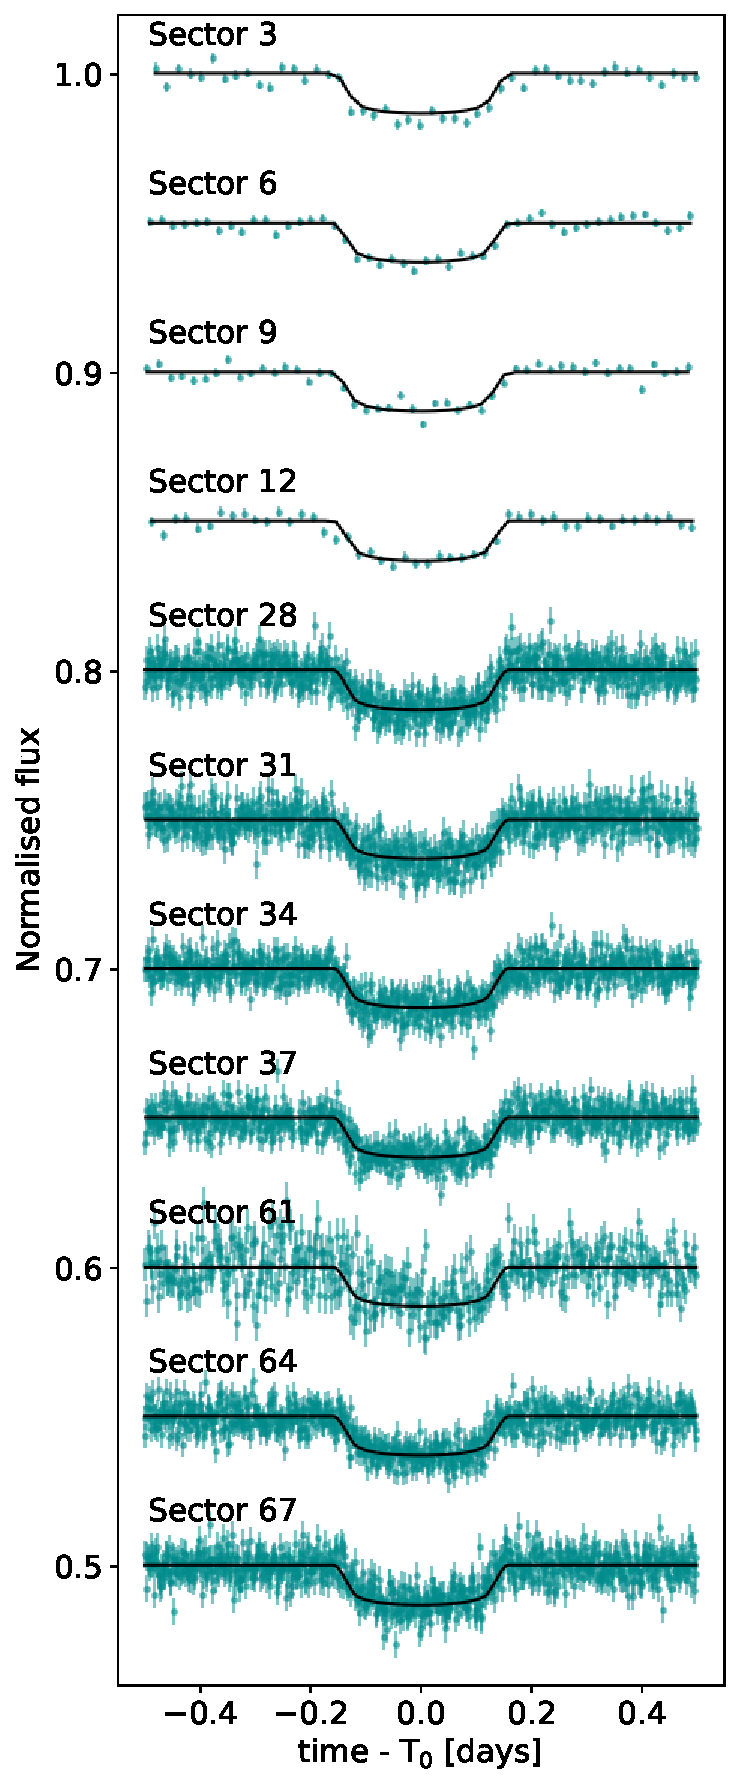
\includegraphics[width=1\linewidth]{transits.pdf}
\caption{Transits of TOI-4504\,c with a model from {\textsc juliet} shifted to have mid-transit at 0 and plotted with vertical offsets.}
\label{trans} 
\end{figure}

\begin{table}[]
\caption{Priors and posteriors for the TTV extraction with {\textsc juliet} for TOI-4504\,c.}
\centering
\label{ttv_juliet}
\begin{tabular}{ccc}
 \hline 
  \hline
Parameter       & Prior                         & Posterior                           \\ \hline
$b$               & $\mathcal{U}$ (0.0,1.0)       & $0.492^{+0.038}_{-0.041}$           \\
$R_p/R_{\star}$               & $\mathcal{U}$ (0.0,1.0)       & $0.108^{+0.001}_{-0.001}$           \\
$q_1$        & $\mathcal{U}$ (0.0,1.0)       & $0.426^{+0.114}_{-0.125}$           \\
$q_2$        & $\mathcal{U}$ (0.0,1.0)       & $0.203^{+0.094}_{-0.091}$           \\
$e$               & fixed 0.0                     & --                                  \\
$\omega$ [$^\circ$]           & fixed 90.0                    & --                                  \\
$\rho_{\star}$ [kg cm$^{-3}$]             & $\mathcal{N}$ (1600,100)      & $1567^{+101}_{-100}$                \\
$m_{\rm dilution}$ & fixed, 1.0                    & --                                  \\
$m_{\rm flux}$     & $\mathcal{N}$ (0.0,0.1)       & $-0.000002^{+0.000012}_{-0.000012}$ \\
$\sigma_w$ [ppm]  & $\mathcal{J}$ (0.1,1000.0)    & $949^{+22}_{-25}$                   \\
$T_0$ [BJD] & $\mathcal{N}$ (2458401.4,0.5) & $2458401.4086^{+0.0032}_{-0.0032}$  \\
$T_1$ [BJD]  & $\mathcal{N}$ (2458483.2,0.5) & $2458483.2110^{+0.0034}_{-0.0034}$  \\
$T_2$ [BJD] & $\mathcal{N}$ (2458565.1,0.5) & $2458565.0902^{+0.0032}_{-0.0033}$  \\
$T_3$ [BJD] & $\mathcal{N}$ (2458647.3,0.5) & $2458647.3328^{+0.0043}_{-0.0045}$  \\
$T_8$ [BJD] & $\mathcal{N}$ (2459065.2,0.5) & $2459065.2370^{+0.0024}_{-0.0023}$  \\
$T_9$ [BJD] & $\mathcal{N}$ (2459148.5,0.5) & $2459148.4782^{+0.0027}_{-0.0026}$  \\
$T_{10}$ [BJD] & $\mathcal{N}$ (2459231.1,0.5) & $2459231.1144^{+0.0021}_{-0.0021}$  \\
$T_{11}$ [BJD]& $\mathcal{N}$ (2459313.3,0.5) & $2459313.2535^{+0.0019}_{-0.0019}$  \\
$T_{19}$ [BJD]& $\mathcal{N}$ (2459976.1,0.5) & $2459976.0493^{+0.0043}_{-0.0045}$  \\
$T_{20}$ [BJD]& $\mathcal{N}$ (2460059.6,0.5) & $2460059.6189^{+0.0023}_{-0.0023}$  \\
$T_{21}$ [BJD]& $\mathcal{N}$ (2460142.6,0.5) & $2460142.6048^{+0.0022}_{-0.0023}$  \\
$P$ [days]               & --                            & $82.97213^{+0.00013}_{-0.00013}$    \\
$t_0$  [BJD]            & --                            & $2458400.3906^{+0.0016}_{-0.0016}$  \\
$a$ [au]               & --                            & $0.3546^{+0.0073}_{-0.0077}$                  \\
$R_p$ [$R_{\rm Jup.}$]   & --                            & $0.99 \pm 0.05$                  \\
$i$ [$^\circ$]   & --                            & $89.69^{+0.02}_{-0.03}$                  \\
\hline
\hline
\end{tabular}
\tablecomments{$P$ was computed as a slope and $t_0$ as an intercept of a least-squares fit to the transit times}
\end{table}
%-------------------------------------------------------------


\begin{figure}
  \centering
  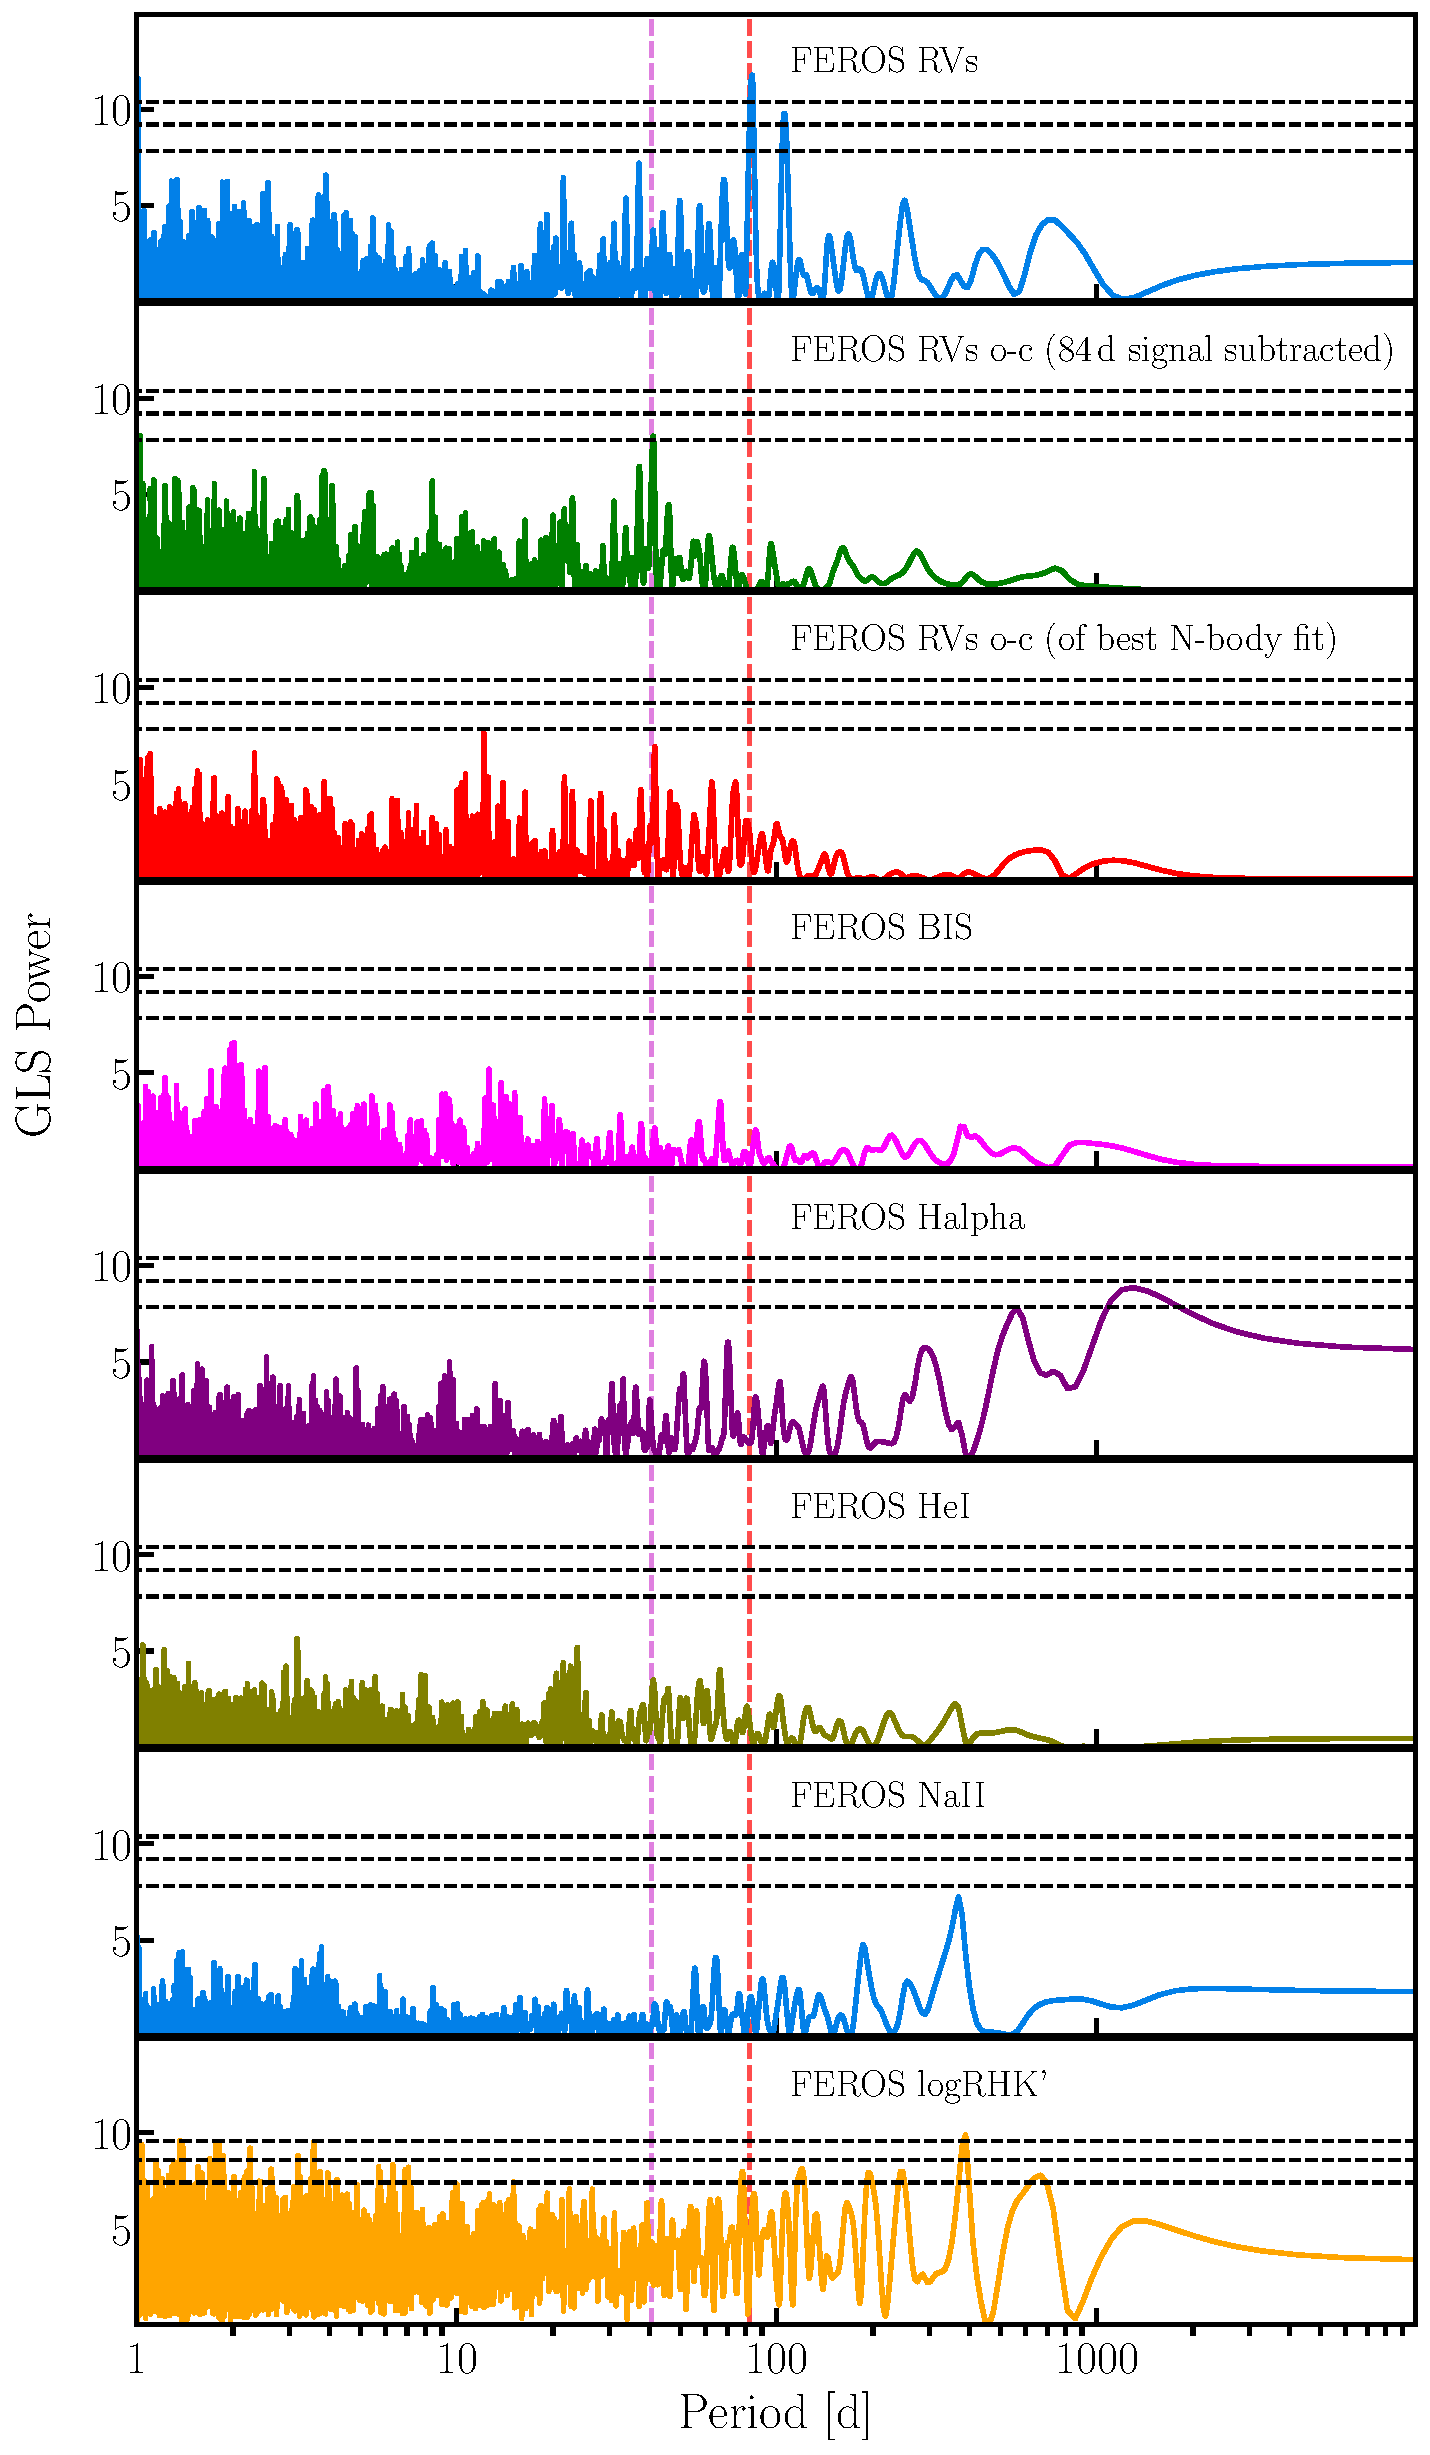
\includegraphics[width=1\linewidth]{GLS_TOI-4504_FEROS_in_Per_2_2.pdf}
  \caption{GLS power spectrum of FEROS spectroscopic products of TOI-4504. From top to bottom panels, as labeled, RVs used in this work, RV residuals after subtracting the dominant signal of TOI-4504\,c at 84\,d, the final the best-fit TTV+RV model residuals, BIS, $\rm{H}_{\alpha}$, He I  Na II, and $\log(R'_{HK})$ activity indicators, respectively. False alarm probability levels of 10\%, 1\%, and 0.1\% are marked with dashed lines, respectively. The red and magenta vertical lines indicate the best-fit periods of the transiting Jovian planet TOI-4504\,c, and the non-transiting TOI-4504\,d, respectively. }
  \label{activity}
\end{figure}


%\subsection{Orbital analysis}
\subsection{Orbital modeling based on TTV and RV data}
\label{nbody_models}

%Our orbital analysis focuses on the TTV data of TOI-4504\,c and the spectroscopic RV data of TOI-4504. 
%The orbital analysis of TOI-4504\,b is based solely on TESS transit fitting using the {\tt juliet} 
%exoplanet fitting package, with orbital parameter results listed in \autoref{02_transit_fit} and illustrated in \autoref{02_transit_fit_fig}.

In this section, we report the orbital analysis results of TOI-4504\,c and its indirectly detected neighbour, which, from now on, we name TOI-4504\,d. We analyzed TOI-4504\,c \& d separately because, as we discussed in \autoref{feros_anaysis}, we were not able to set constraints on the mass of the transiting planet TOI-4504\,b with the FEROS RV data, nor with detailed three-planet N-body modeling of the TESS transits and TTVs 
separately or together with the RV data. We note in passing that we performed a three-planet orbital analysis including TOI-4504\,b, but including TOI-4504\,b did not significantly improve the fit compared to the models considering only TOI-4504\,c \& d, and thus shall not be discussed in this work. 


We conducted a joint global orbital analysis using broad priors to explore the parameter space consistent with the TTV and RV data for TOI-4504, using the {\textsc Exo-Striker}\footnote{Available at \url{https://github.com/3fon3fonov/exostriker}} exoplanet modeling toolbox \citep{exostriker}. Our fitting scheme followed a more targeted N-body orbital fit once the consistent parameter space had been identified.
Taking the gravitational 
interactions between TOI-4504\,c \& d into account, the {\textsc Exo-Striker} uses an internal RV dynamical model, whereas the TTV model is wrapped around the \mbox{\textsc TTVfast} package \citep{Deck2014}. We follow a very similar TTV+RV N-body fitting approach, used by \citet{TOI-2202} for the TOI-2202 system, which is similar to TOI-4504 in many aspects. We refer the reader to \citet{TOI-2202} for more details, and below we summarize our fitting methods, used parameters, adopted priors, and more results relevant to our modeling cascade, which reveal the orbital and physical parameters of the TOI-4504\,c \& d pair.

The fitted parameters for each planet in the TTV+RV model were the RV semi-amplitude $K_{\rm c,d}$ and the osculating planetary orbital period $P_{\rm c,d}$. The eccentricities $e_{\rm c,d}$, arguments of periastron $\omega_{\rm c,d}$, and mean anomalies $M_{\rm c,d}$ were derived using the parameterization $h = e\sin\omega$, $k = e\cos\omega$, and $\lambda = \omega + M$, which is more efficient for orbits with small eccentricities \citep{Tan2013}. 
Since we know that the perturber planet is not transiting, we  assumed a non-coplanar, mutually inclined orbital geometry and fitted for the orbital inclinations $i_{\rm c,d}$ and the difference between the longitudes of the ascending nodes $\Delta\Omega_{\rm d - c}$ = $\Omega_{\rm d}$ - $\Omega_{\rm c}$, where the mutual inclination comes following the expression:
\begin{equation}
\Delta i = \arccos[\cos(i_d)\cos(i_{c})+\sin(i_d)\sin(i_{c})\cos(\Delta\Omega)] .
\label{eq:deltai}
\end{equation}

\noindent
Since only $\Delta\Omega$ is important, we kept $\Omega_{\rm d}$ fixed to 0$^{\circ}$, and we fit for $\Omega_{\rm c}$.

All osculating parameters in our N-body fitting were defined in the Jacobi coordinate system, which is standard practice for multiple-planet systems \citep[][]{Lee2003}, and are valid for the reference epoch BJD = 2458400.0, arbitrarily chosen before the first {\it TESS} transit of TOI-4504\,c.
Additionally, for the FEROS RV data, we fitted the RV offset and RV jitter parameters \citep[see,][]{Baluev2009}. For the stellar mass of TOI-4504, we used 0.885 $M_{\odot}$, which, together with the fitted parameters, was converted to dynamical planetary masses $m_{\rm c,d}$ needed to construct the N-body model. The numerical time step in the dynamical model was set to 0.5 days, which is sufficiently small for accurate modeling of the system.

 
\begin{figure*}
  \centering
  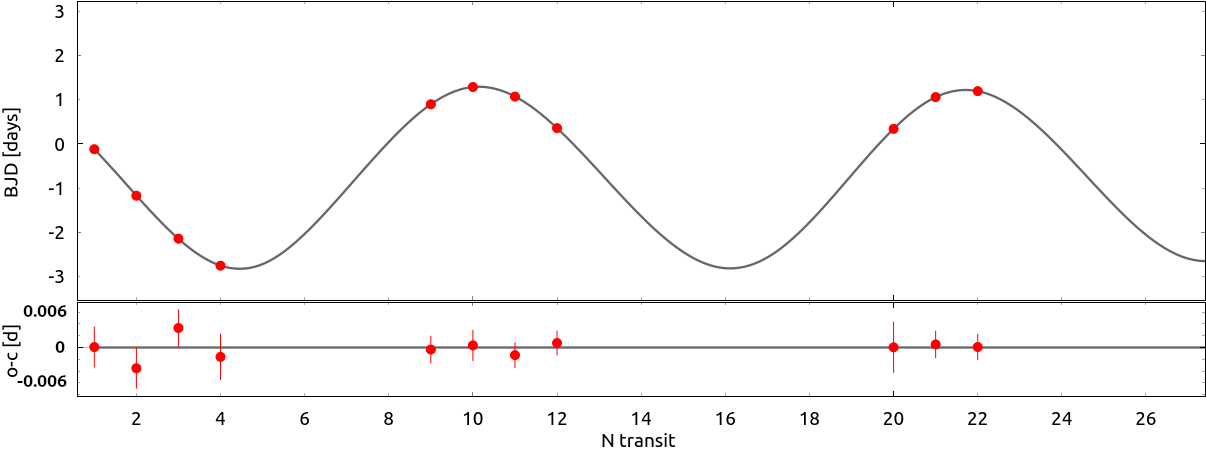
\includegraphics[width=1\linewidth]{ttv_2.png}
    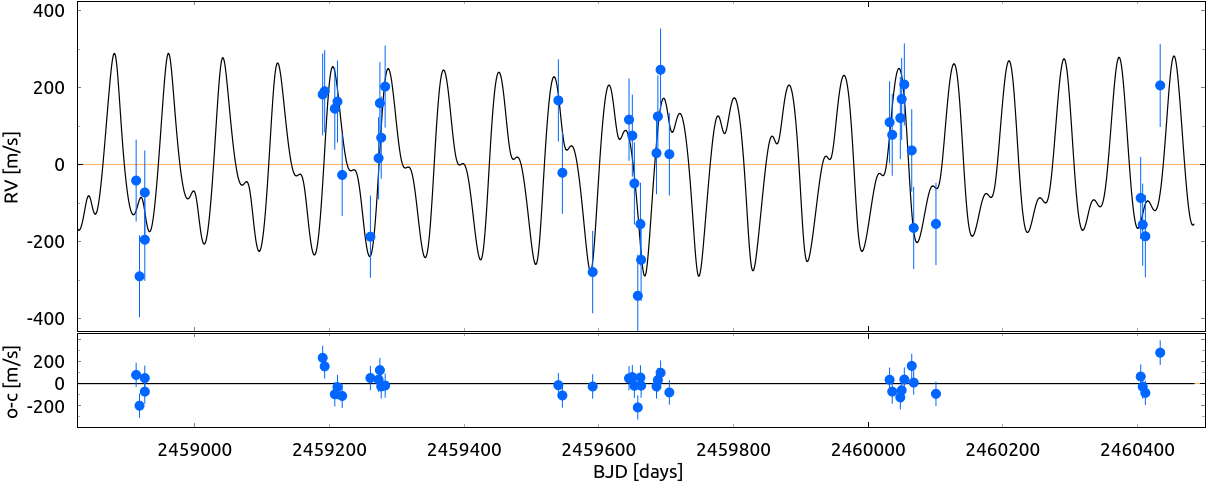
\includegraphics[width=1\linewidth]{RVs.png}


  \caption{TESS TTV time series of TOI-4504\,c and a model consistent with two Jovian-mass planets with periods close to the 2:1 MMR commensurability, with the non-transiting planet being interior (top panel). The TTV signal is expressed as the deviation of the {\it TESS} transit events with respect to the mean osculating Period of TOI-4504\,c, which have a large semi-amplitude of $\sim$ 2\,d and super-period of 946.5\,d. The bottom sub-panel shows the TTVs residuals. The main bottom panel shows the Doppler component of the same model fitted to the FEROS RV data. The bottom sub-panel shows the RV residuals.}
  \label{TTVs}
\end{figure*}
 

    \begin{figure}
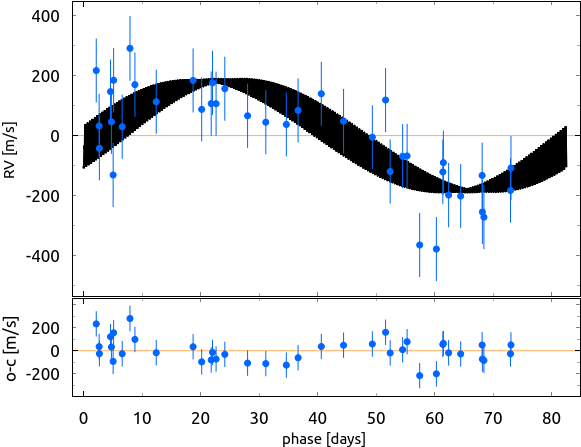
\includegraphics[width=0.49\linewidth]{TOI-4504_c_ph.png}\put(-45,80){\scriptsize TOI-4504\,c }
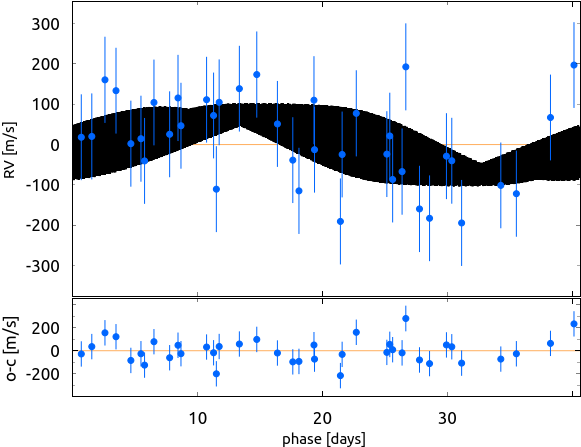
\includegraphics[width=0.49\linewidth]{TOI-4504_d_ph.png}\put(-45,80){\scriptsize TOI-4504\,d }\\
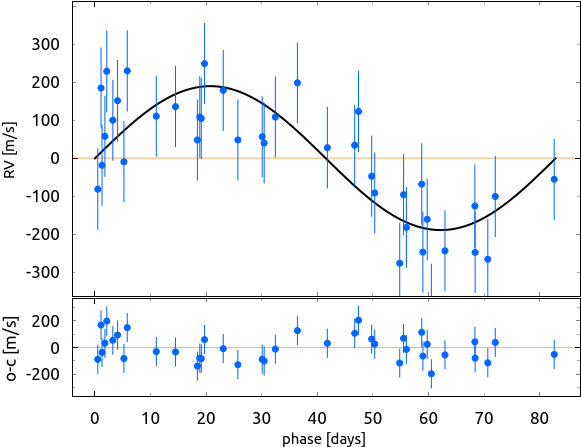
\includegraphics[width=0.49\linewidth]{TOI-4504_c_ph_mean_period.png}\put(-45,80){\scriptsize TOI-4504\,c }
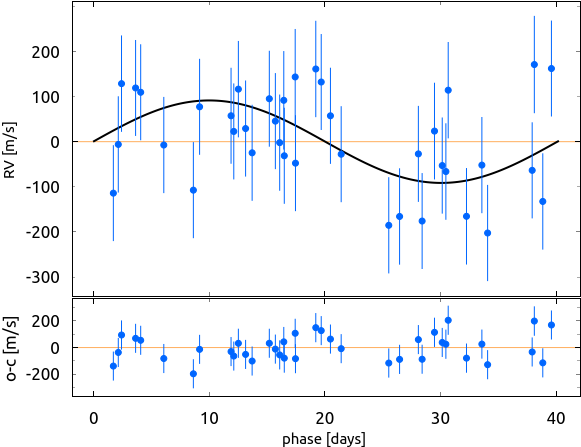
\includegraphics[width=0.49\linewidth]{TOI-4504_d_ph_mean_period.png}\put(-45,80){\scriptsize TOI-4504\,d }



\caption{Phased RV signals for the planets TOI-4504\,c and d. The top two 
panels display the planetary signals along with the osculating N-body model, phased 
to the best-fit periods from \autoref{NS_params}, valid for BJD = 2458400.0. The 
bottom two panels illustrate the same planetary signals, phased to the mean osculation periods derived from the TTV+RV model.}
\label{phased} 
\end{figure}

\begin{table*}[ht!]
\caption{{MCMC sampling priors, posteriors, and the optimum $-\ln\mathcal{L}$ orbital parameters of the two-planet system derived by joint N-body modeling of TTVs (TESS) and RVs (FEROS).}}
\label{NS_params}
\centering
 \begin{adjustwidth}{-2cm}{}
 \resizebox{0.83\textheight}{!}
 {\begin{minipage}{1.1\textwidth}

\begin{tabular}{lrrrrrrrrrrrr}     % 2 columns

\hline\hline  \noalign{\vskip 0.7mm}

%\makebox[0.1\textwidth][l]{\hspace{60 mm}$\sim$2:1 MMR fit      \hspace{60 mm} $\sim$3:1 MMR fit  \hspace{1.5 mm} } \\
%\cline{2-5}\cline{7-10}\noalign{\vskip 0.9mm}   
\makebox[0.1\textwidth][l]{\hspace{45 mm} Median and $1\sigma$  \hspace{15 mm} Max. $-\ln\mathcal{L}$     \hspace{30 mm} Adopted priors  \hspace{10 mm} \hspace{1.5 mm} } \\
\cline{1-9}\noalign{\vskip 0.7mm}   


Parameter &\hspace{10.0 mm} Planet d & Planet c &  & Planet d & Planet c  & & \hspace{10.0 mm}Planet d & Planet c  \\
%   \hline \noalign{\vskip 0.7mm}
\cline{1-9}\noalign{\vskip 0.7mm}   
 
$K$  [m\,s$^{-1}$]            & 90.8366$_{-2.5466}^{+1.8812}$ & 190.8921$_{-6.2119}^{+4.7269}$ &  
                              & 91.3360 & 189.2623 &
                              & $\mathcal{U}$(80.0, 140.0) & $\mathcal{U}$(150.0, 250.0)   \\ \noalign{\vskip 0.9mm}

$P$  [days]                    & 40.5634$_{-0.0368}^{+0.0363}$ & 82.5438$_{-0.0176}^{+0.0150}$ & 
                              & 40.5586 & 82.5383 &  
                              & $\mathcal{U}$(40.2, 40.6) & $\mathcal{U}$(81.0, 83.0)   \\ \noalign{\vskip 0.9mm}
                              
$e \sin(\omega)$               & 0.0439$_{-0.0011}^{+0.0010}$ & -0.0320$_{-0.0016}^{+0.0014}$ &
                              & 0.0441 & -0.0320 &  
                              & $\mathcal{U}$( -0.1, 0.1) & $\mathcal{U}$( -0.1, 0.1)   \\ \noalign{\vskip 0.9mm}

$e \cos(\omega)$               & -0.0064$_{-0.0047}^{+0.0039}$ & 0.0005$_{-0.0013}^{+0.0011}$ &
                              & -0.0027 & -0.0009 &  
                              & $\mathcal{U}$( -0.1, 0.1) & $\mathcal{U}$( -0.1, 0.1)   \\ \noalign{\vskip 0.9mm}

$\lambda$  [deg]               & 9.89$_{-2.43}^{+3.45}$  & 83.97$_{-0.15}^{+0.12}$ &
                              & 14.11 & 83.80 &   
                              & $\mathcal{U}$(0.0, 360.0) & $\mathcal{U}$(70.0, 110.0)  \\ \noalign{\vskip 0.9mm}

$i$  [deg]               & 85.00$_{-0.30}^{+0.28}$  & 89.69$_{-0.03}^{+0.03}$ &
                              & 84.74 & 89.68 &   
                              & $\mathcal{N}$(      86.0,    3.0)& $\mathcal{N}$(      89.7,    0.1)\\ \noalign{\vskip 0.9mm}

$\Delta\Omega$  [deg]               & $\dots$  & 0.0$_{-1.0}^{+0.9}$ &
                              & $\dots$ & -0.8&   
                              & $\dots$ & $\mathcal{N}$(0.0, 30.0)  \\ \noalign{\vskip 0.9mm}
                              
 

RV$_{\rm off.}$ FEROS  [m\,s$^{-1}$]  & $\dots$  & 2067.0517$_{-14.8783}^{+14.2161}$  &     & $\dots$ &  2064.9642    &      & $\dots$ & $\mathcal{U}$(1900.0, 2200.0)  \\ \noalign{\vskip 0.9mm}
RV$_{\rm jit.}$ FEROS  [m\,s$^{-1}$]  & $\dots$ & 103.3721$_{-7.0042}^{+13.8367}$   &  &  $\dots$ & 104.6664     &         & $\dots$ & $\mathcal{U}$(1.0, 150.0)  \\ \noalign{\vskip 0.9mm}


%0.044501364011659356 - 0.0008769572039779849 + 0.0010189815376304284
%0.03200772244443349 - 0.001433813572219677 + 0.0016183100106932358
%98.26518773366644 - 5.075105095143584 + 6.066885055286903
%270.89158998397454 - 2.248731914702887 + 2.039263823617432
%271.61782056744033 - 7.516692564398284 + 7.35468787912032
%173.075514117695 - 1.9147053793222994 + 2.104311697066464
%4.725536193322315 - 0.254677033676197 + 0.34625921359118994

$e$                             & 0.0445$_{-0.0009}^{+0.0010}$ & 0.0320$_{-0.0014}^{+0.0016}$ &
                              & 0.0441 & 0.0320 &  
                              & (derived)  & (derived)   \\ \noalign{\vskip 0.9mm}

$\omega$ [deg]                & 98.3$_{-5.1}^{+6.1}$ & 270.9$_{-2.2}^{+2.0}$ &
                              & 93.5 & 268.4&  
                              & (derived)  & (derived)   \\ \noalign{\vskip 0.9mm}

$M_0$  [deg]                 & 271.6$_{-7.5}^{+7.3}$  & 173.1$_{-1.9}^{+2.1}$ &
                              & 280.6 & 175.4 &   
                              & (derived)  & (derived)   \\ \noalign{\vskip 0.9mm}

$\Delta i$  [deg]             & $\dots$ & 4.7$_{-0.3}^{+0.3}$   &  
                              &   $\dots$ & 5.0 &    
                              &     $\dots$  & (derived) & \\ \noalign{\vskip 0.9mm}



$m_p$  [M$_{\rm Jup.}$]          & 1.4166$_{-0.0647}^{+0.0651}$  & 3.7672$_{-0.1822}^{+0.1810}$ & 
                              & 1.4294 & 3.7494 &     
                              & (derived) & (derived)   \\ \noalign{\vskip 0.9mm}

$a_p$  [au]                     & 0.2219$_{-0.0043}^{+0.0041}$  & 0.3569$_{-0.0069}^{+0.0066}$  &  
                              & 0.2219 & 0.3569 &     
                              & (derived) & (derived)   \\ \noalign{\vskip 0.9mm}
 
\hline \hline \noalign{\vskip 0.7mm}

\end{tabular}
\end{minipage}}
\end{adjustwidth}
\tablecomments{The orbital elements are in the Jacobi frame and are valid for epoch BJD = 2458400.0. The adopted priors are listed in the right-most columns, and their meanings are $\mathcal{U}$ -- Uniform, and $\mathcal{N}$ -- Gaussian priors.
%and $\mathcal{J}$ -- Jeffrey's (log-uniform) priors. 
The derived planetary posterior parameters of $a$, and $m$ are calculated by considering the stellar parameter uncertainties.}
\end{table*}


\begin{figure*}


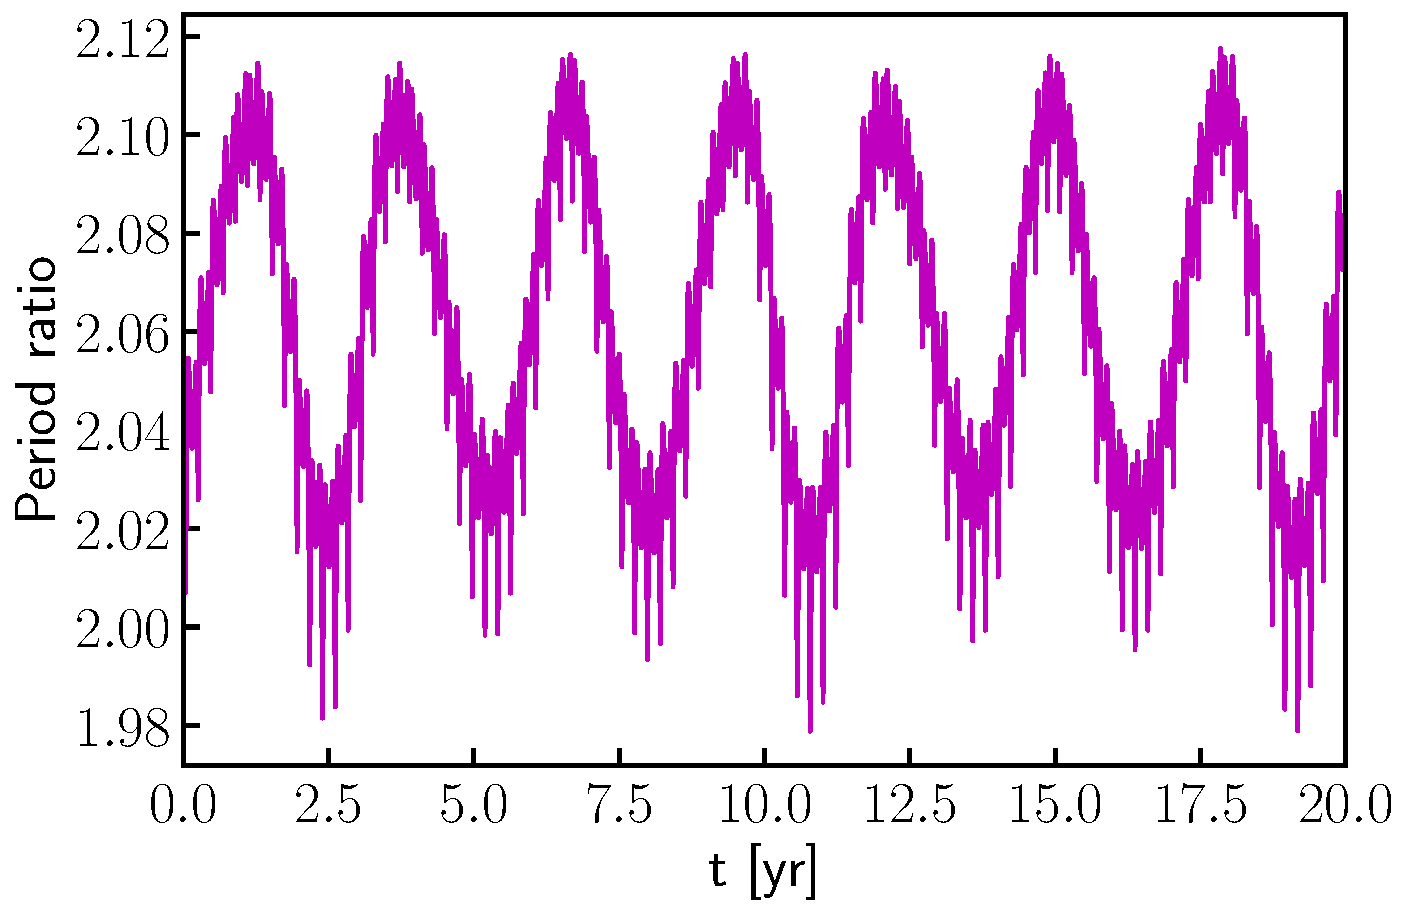
\includegraphics[width=9cm]{evol_Prat.pdf}
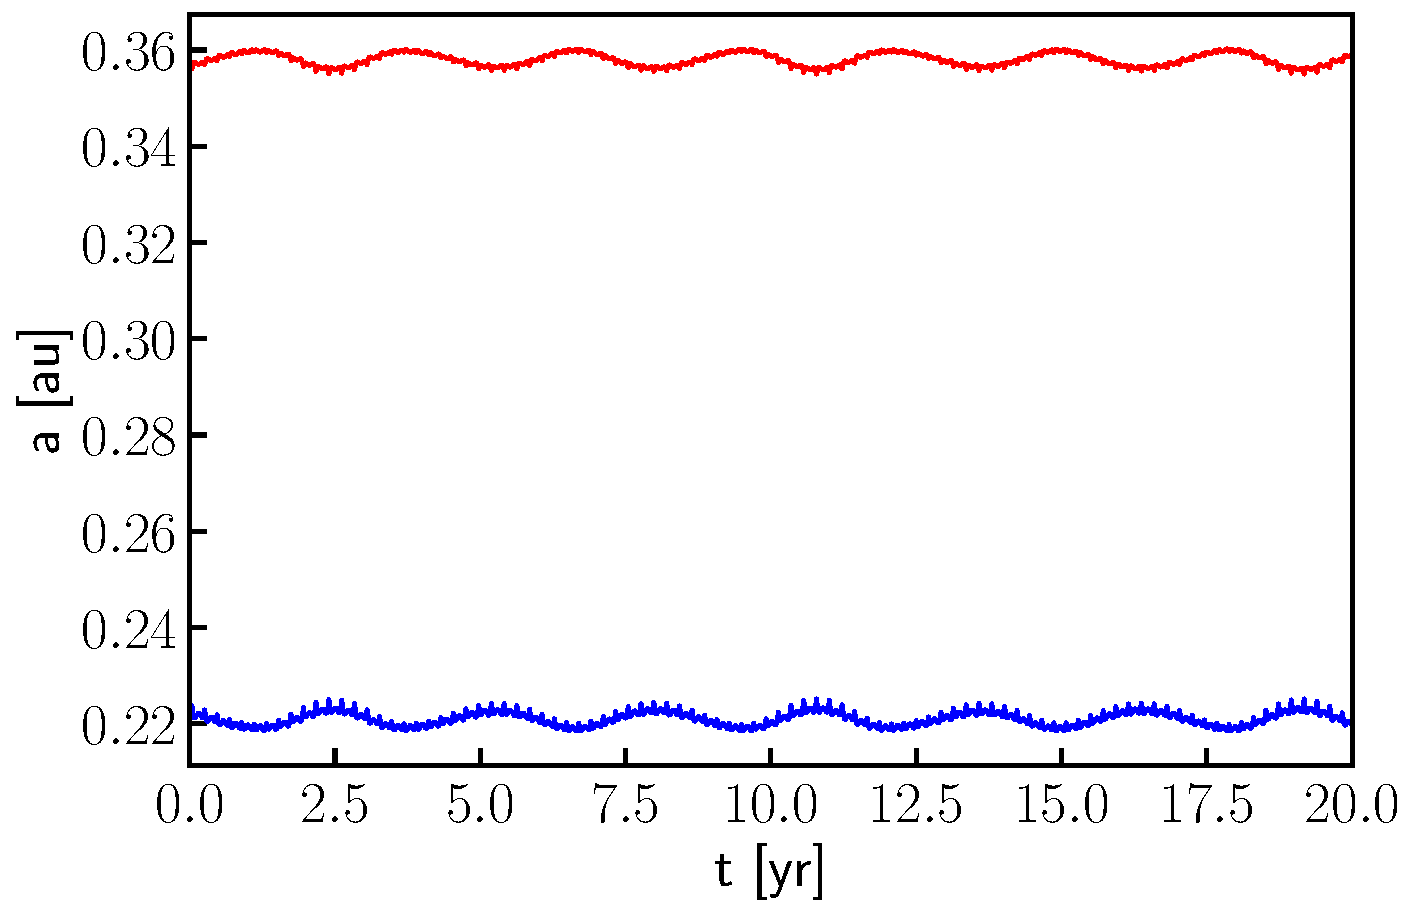
\includegraphics[width=9cm]{evol_a.pdf} \\
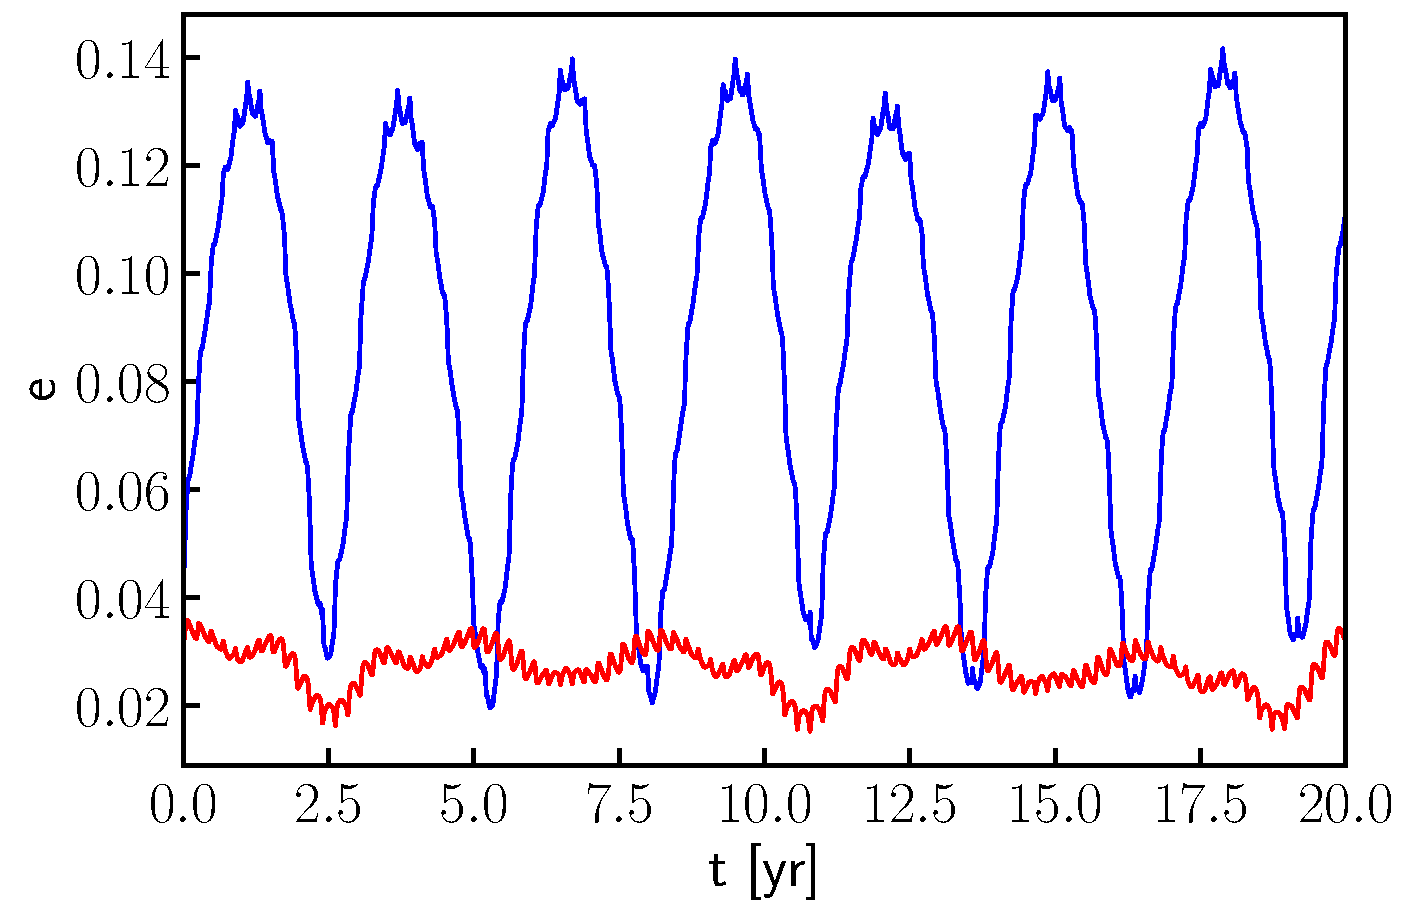
\includegraphics[width=9cm]{evol_e.pdf} 
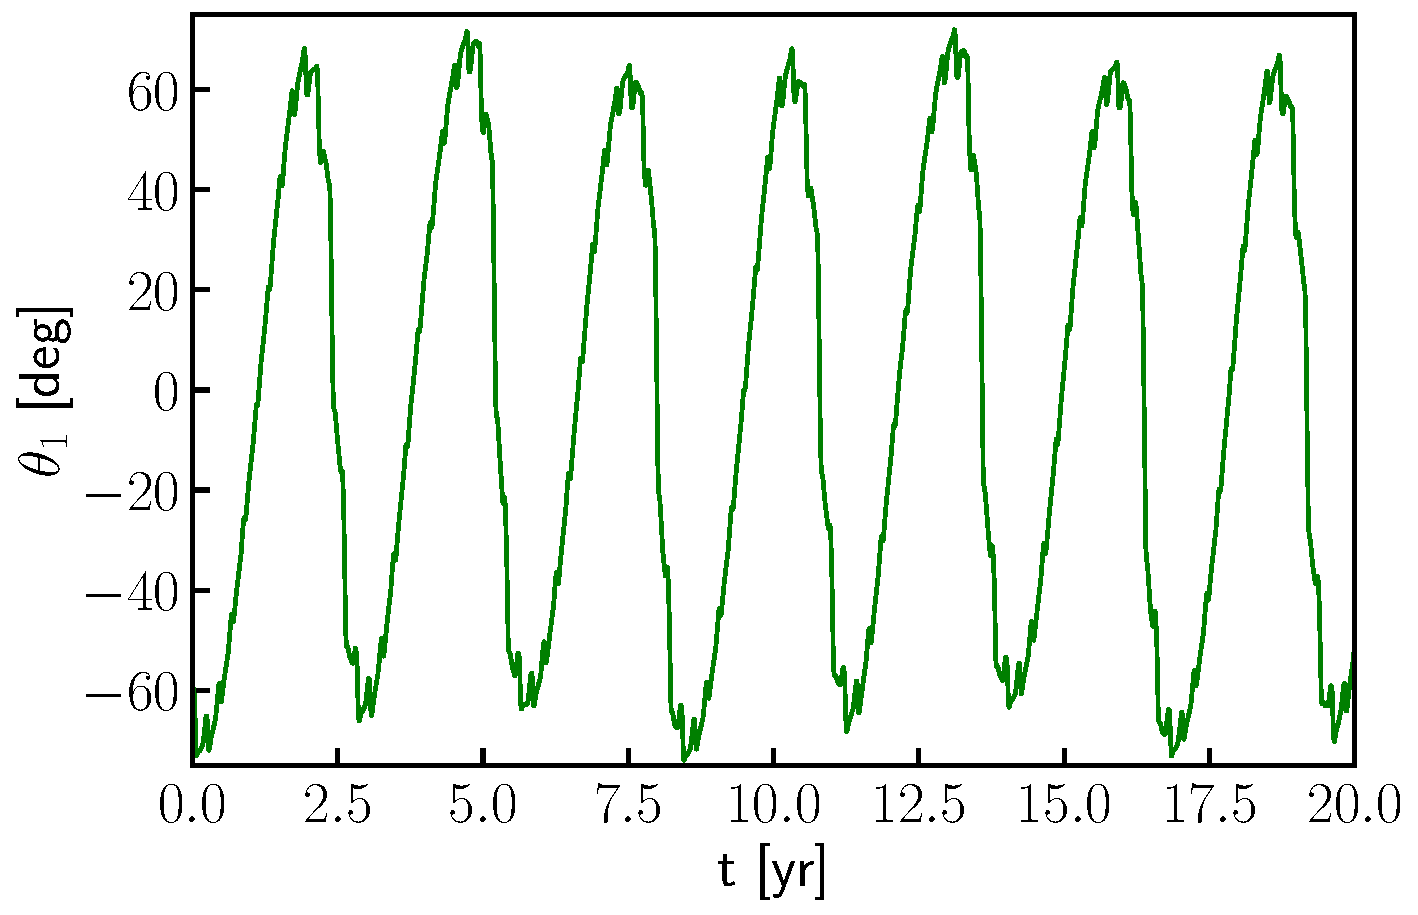
\includegraphics[width=9cm]{evol_t1.pdf} 
\caption{Orbital evolution of the best TTV+RV N-body model of the TOI-4504 system for a short extent of 20\,yr long N-body simulation using the {\textsc Exo-Striker}. The top row from left to right panels shows the evolution of the planetary period ratio ($P_{\rm c} / P_{\rm d}$) (magenta) and the evolution of the semi-major axes $a_{\rm c}$ (red) and $a_{\rm d}$ (blue), respectively. The bottom row from left to right panels shows the evolution of the eccentricities $e_{\rm c}$ (red) and $e_{\rm d}$ (blue) and $\theta_1$ (green), which librates around 0$^{\circ}$ with amplitude of $\sim$ 65$^{\circ}$, respectively. }
\label{evol_plot} 
\end{figure*}

We first used a global Nested Sampling (NS) parameter search \citep{Skilling2004} via the {\textsc dynesty} sampler \citep{Speagle2020}. We employed a Static-NS setup with 500 "live points" per fitted parameter \citep[see][for details]{Speagle2020}, to explore a wide parameter space of 
eccentricities, masses, and periods for the "yet-to-be detected" planet TOI-4504\,d, assuming it could be either interior or exterior to TOI-4504\,c. For TOI-4504\,c, the prior parameter range estimates were taken from our GLS and TTV extraction analysis, making the parameter search more constrained. The adopted prior ranges for TOI-4504\,d \& c are listed in \autoref{globalNS}. Our results showed very poor fits when TOI-4504\,d was assumed to be exterior. In contrast, good fits were found in the resulting posterior probability distribution analysis when the planet was considered interior. As indicated in \autoref{Nest_samp_ttv}, the posteriors are multimodal but firmly converge with TOI-4504\,d being an interior planet in the 2:1 period ratio commensurability.



As a next step, we used the NS posteriors and the best $-\ln\mathcal{L}$ NS solution as an initial guess for a more targeted Simplex optimization \citep{NelderMead}, aiming to find the optimal $-\ln\mathcal{L}$ best-fit solution. This was followed by an affine-invariant ensemble Markov Chain Monte Carlo (MCMC) sampler \citep{Goodman2010} via the \texttt{emcee} package \citep{emcee} to build the parameter posteriors and obtain parameter uncertainties.

\autoref{TTVs} shows our best joint fit to the TTVs and RVs, whereas 
\autoref{mcmc_posteriors} displays the MCMC posteriors drawn around the best fit. \autoref{NS_params} lists the best fit in terms of optimal $-\ln\mathcal{L}$ shown in \autoref{TTVs}, the median orbital parameters and their uncertainties extracted from our MCMC posteriors, and the used priors.

\autoref{phased} shows the phased RV planet signals of TOI-4504\,c and d, respectively.
The top two panels of \autoref{phased} show the phased planetary periods to the N-body fit, which, due to the dynamical nature of the model are strong osculating. In contrast, the bottom two panels provide a clearer representation of the RV signals, phased to the main osculation periods from the TTV+RV N-body model, which we estimate to be 82.5438$_{-0.0176}^{+0.0150}$\,d, and 40.5634$_{-0.0368}^{+0.0363}$\,d for TOI-4504\,c and d, respectively.
We conclude that the TTVs from TESS and the RV data from FEROS suggest the presence of a massive pair of Jovian planets with osculating periods of $P_{\rm d}$ = 40.5634$_{-0.0368}^{+0.0365}$\,days and $P_{\rm c}$ = 82.5438$_{-0.0150}^{+0.0176}$\,days, and small but significantly non-zero eccentricities of $e_{\rm d}$ = 0.0445$_{-0.0009}^{+0.0010}$ and $e_{\rm c}$ = 0.0320$_{-0.0014}^{+0.0016}$, valid for reference epoch of BJD = 2458400.0. We obtain dynamical masses of $m_{\rm d}$ = 1.417$_{-0.065}^{+0.065}$\,M$_{\rm Jup}$ and $m_{\rm c}$ = 3.767$_{-0.181}^{+0.182}$\,M$_{\rm Jup}$ for TOI-4504\,d and TOI-4504\,c, respectively. The mutual inclination between the two planets suggests a non-coplanar configuration with $\Delta i$ = 4.7$_{-0.3}^{+0.3}$ degrees, which agrees with the fact that TOI-4504\,d is not transiting.

 

\subsection{Dynamics and long-term stability}
\label{sec4.3}

%We inspected the Angular Momentum Deficit \citep[AMD;][]{Laskar2017} stability criteria of 
%the TOI-4504 system and found that our posteriors are predicted to be long-term stable. 
%However, the AMD criteria only serve as a proxy for long-term stability and do not fully 
%account for the system's MMR dynamics. Therefore, 

We performed N-body simulations to study the long-term stability 
and dynamical evolution of the TOI-4504 system. For this test, 
we again ignored the innermost planet TOI-4504\,b, since, even if its 
dynamical mass is in the Neptune mass regime, its overall mutual 
Hill distance with TOI-4504\,d would be $\sim$ 17 R$_{\rm Hill,m}$ \citep[see,][]{Gladman1993}, thus would result in minimal dynamical interactions with the outer pair. 
Additionally, including TOI-4504\,b would require using a very 
small time step of approximately 30 minutes (1/100 of the orbital period of the planet) to achieve accurate orbital dynamics, which would be computationally expensive.

Our study of the long-term dynamics and possible MMR dynamics in the system adopted the same N-body numerical setup used in our recent analyses of the TOI-2202 \citep{TOI-2202} and TOI-2525 \citep{Trifonov2023} systems, which share similar 
physical and orbital characteristics with the Jovian pair of 
TOI-4504. We conducted numerical integrations using a custom 
version of the Wisdom-Holman N-body integrator \citep{Wisdom1991}, 
specifically tailored for long-term stability analyses of exoplanetary systems in Jacobi orbital elements. Integrated natively within the {\sc Exo-Striker} toolbox, this N-body integrator allows direct injection of posterior samples in Jacobi coordinates, thereby avoiding the additional coordinate transformations typically required by other publicly available N-body integrators.
We 
tested the stability of the TOI-4504 system for a maximum of 10 million years 
with a time step of 0.5 days for 10,000 randomly chosen samples 
from the achieved orbital parameters of the TTV+RV MCMC parameter 
posteriors. For each sample integration and at each numerical time step, we monitor the planetary semi-major axes, ensuring they do 
not deviate by more than 20\% from their initial values; any orbit 
exceeding this threshold is considered unstable, resulting in the 
termination of the integration. Additionally, integrations are flagged 
as unstable and terminated if eccentricity values become sufficiently 
excited to orbit-crossing configurations. Further details on our 
stability criteria are provided in \citet{TOI-2202}.



We found that all examined parameters are long-term stable. From the numerical evolution, we built a posterior distribution of some of the important dynamical properties of the system, such as the mean period ratio $P_{\rm rat.}$, mean eccentricities $\hat e_{\rm d}$, $\hat e_{\rm c}$, their peak-to-peak amplitudes $e_{\rm d}$, $e_{\rm c}$, the dynamical masses of the planets $m_{\rm d}$, $m_{\rm c}$, and the orbital semi-major axes $a_{\rm d}$, $a_{\rm c}$, as in \citet{wine5,Trifonov2023}. We also collected posterior distributions of the resonance angles defined as:

\begin{equation}
\Delta\omega = \omega_{\rm c} - \omega_{\rm d}
\label{eq1}
\end{equation}

\noindent
which is the secular apsidal angle, and:

\begin{equation}
\theta_1 =  \lambda_{\rm c} - 2\lambda_{\rm d} + \omega_{\rm c},~~~~~~\theta_2 =  \lambda_{\rm c} - 2\lambda_{\rm d} + \omega_{\rm d}
\label{eq2}
\end{equation}

\noindent
are the first-order eccentricity-type 2:1 MMR angles, of which at least one must librate 
around a fixed angle to claim the system in an MMR \citep[see][]{Lee2004}. 

%\autoref{dyn_samp} shows that the 
We find that the TOI-4504 system exhibits moderate eccentricity evolution, with the less massive planet, TOI-4504\,d, showing larger eccentricity variations, from 0.02 to 0.12. In all cases, the period ratio oscillates around $\sim$ 2.06, slightly above the exact 2:1 period ratio. The angles $\theta_2$ and $\Delta\omega$ circulate between  0$^\circ$ and 360$^\circ$, while $\theta_1$ librates around 0$^\circ$ with a mean semi-amplitude of 73$^\circ$ for all integrated samples. This libration of $\theta_1$ in all samples implies that the massive planets in the TOI-4504 system are involved in a 2:1 MMR, despite the minor offset in period ratio, which, given the strong dynamical interactions, is needed to maintain the resonance.


\autoref{evol_plot} shows an example of a 20-year extent of the orbital evolution simulation started from the best fit (i.e., maximum $-\ln\mathcal{L}$; see \autoref{NS_params}). We show the evolution of the mutual period ratio $P_{\rm rat.}$, the eccentricities $e_{\rm c}$ and $e_{\rm d}$, and the first-order eccentricity-type 2:1 MMR angle $\theta_1$. The evolution of the model based on the best-fit parameters is indicative of the orbital evolution of the posterior samples. The libration of $\theta_1$ is sufficient to conclude that the TOI-4504 Jovian pair is involved in a 2:1 MMR \citep[][]{Lee2004}. 


\subsection{Internal composition of TOI-4504\,c}
For TOI-4504\,c, we computed planet interior models and their thermal evolution with {\textsc MESA} \citep{mesa1,mesa2}, following the implementation described in \cite{jones2024}. In this case, we modeled the planet with the heavy elements condensed in an inert isodensity core surrounded by a pure gas (H/He) envelope.  
We assumed a 1:1 mixture of rock and ice for the core, with their density obtained from the $\rho-P$ relations 
presented in \cite{hubb1989}. The density of the mixture was computed using the additive volume law. 
We evolved different models with different masses of the core and compared them with the current position of TOI-4504\,c 
in the radius-age diagram. \autoref{internal_comp} shows different models that agree at the 1-$\sigma$ level with the current
radius of the planet. These results correspond to a planet metallicity of Z$_p$  = 0.21$^{+0.07}_{-0.09}$, and a      
corresponding heavy-element enrichment with respect to the host star of Z$_p$/Z$_\star$ = 9.6 $^{+3.1}_{-4.1}$.



%-------------------------------------------------------------
\section{Summary and conclusions}
\label{sec5}

In this work, we report the discovery and orbital analysis of a multi-planetary system orbiting the K-dwarf star TOI-4504. We analyzed available photometric data from TESS and conducted follow-up spectroscopic observations with FEROS to constrain the orbital and physical parameters of the detected exoplanets. We confirm two transiting planets, TOI-4504\,b and TOI-4504\,c, and we discover an additional Jovian-mass exoplanet TOI-4504\,d, based on the dynamical perturbations induced on TOI-4504\,c, evidenced by strong TTVs with the largest ever detected semi-amplitude of $\simeq$ 2 days.
Our analysis indicates that the TOI-4504 system consists of a hot sub-Neptune and two warm Jovian planets in a 2:1 MMR. %, making it one of the most massive and compact multiple-planet systems.



\begin{figure}
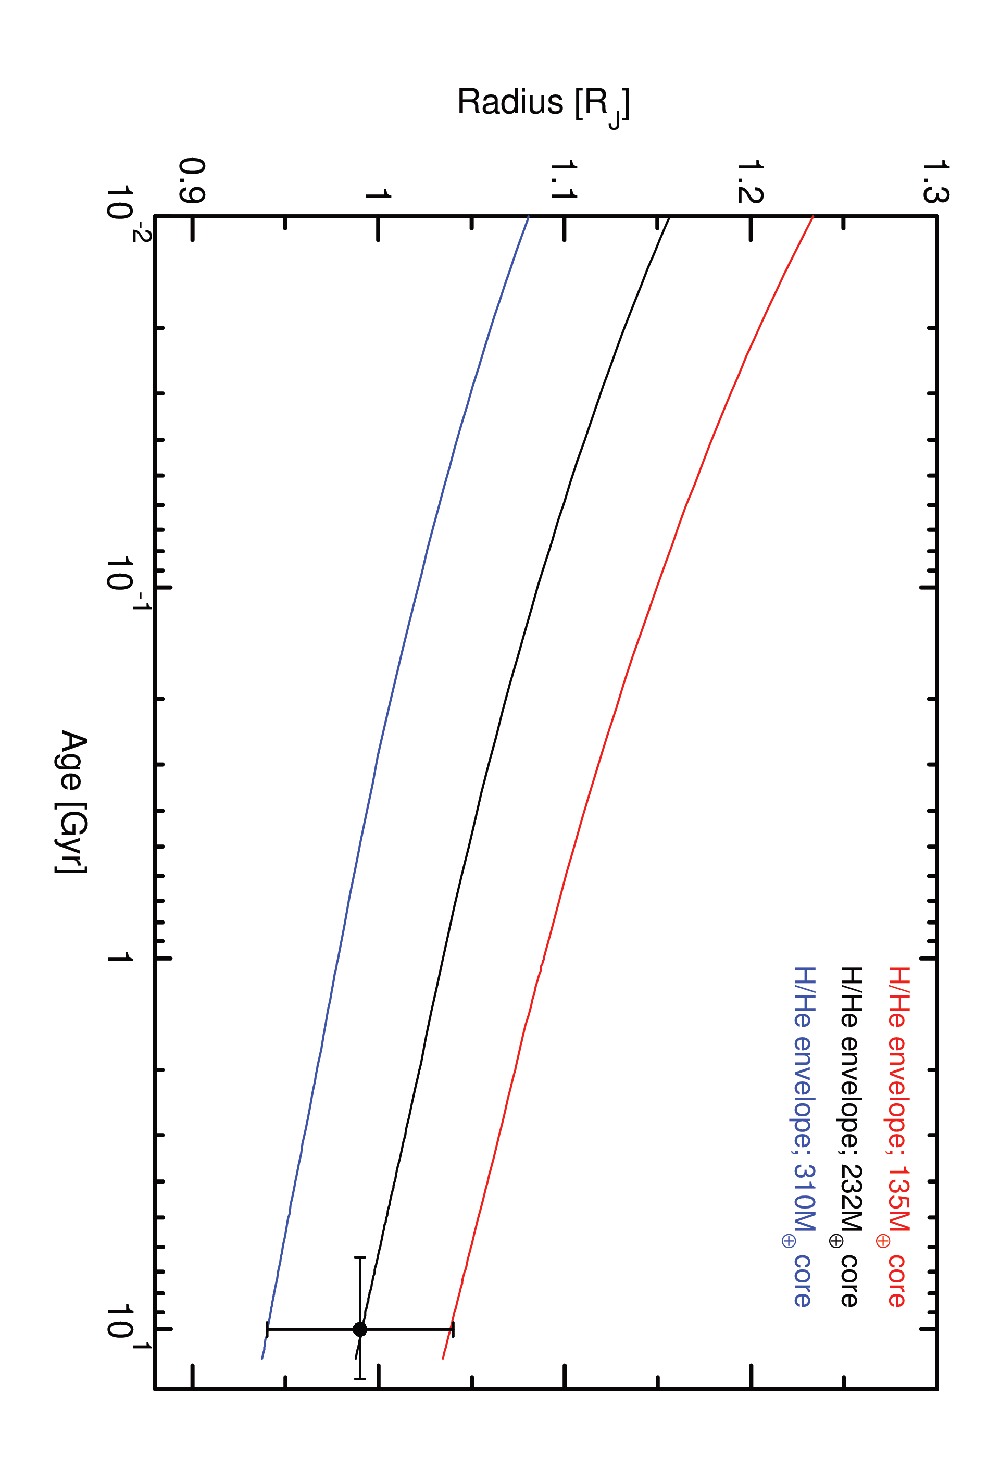
\includegraphics[width=0.72\linewidth,angle=90]{age_rad_TOI4504.pdf}
\caption{Position of TOI-4504\,c in the age-radius diagram (black dot). Three different models with an isodensity core ($\rho$ =  15 [g\,cm$^3$]) with different masses, and surrounded by an H/He envelope are overplotted (solid lines). }
\label{internal_comp} 
\end{figure}

The innermost planet, TOI-4504\,b, was only detected in the TESS photometry with a period of 2.42614$^{+0.00014}_{-0.00013}$ days and an estimated radius of $2.69 \pm 0.19$ R$_{\oplus}$. The precision of our RVs is not enough to measure the mass of this potential $\sim$10 M$_{\oplus}$ sub-Neptune \citep{muller:2024}.
TOI-4504\,b is a potentially interesting candidate for further 
characterization of its possible atmospheric composition with JWST \citep[e.g.,][]{madhusudhan:2023,holmberg:2024}. TOI-4504\,b has a predicted transmission spectroscopy metric of $\sim$20 \citep{tsm} and is among the handful of hot sub-Neptunes transiting solar type stars that can be observed with NIRSpec/Prism avoiding saturation, which allows obtaining a transmission spectrum with a wide wavelength coverage (0.6--5.3 $\mu m$ s) from a single transit.

%planet c mean P = 82.85406206298813 - 0.010098328258592915 + 0.009121871731224473
%planet d mean P = 40.171602230253555 - 0.015802770022247614 + 0.014531354307898425


TOI-4504\,c was detected in the TESS data and FEROS RVs and has a period of 82.5438$_{-0.0176}^{+0.0150}$ days valid for epoch BJD = 2458400, a mean orbital period of  82.8540$_{-0.0010}^{+0.0009}$\,days, an estimated radius of $0.9897 \pm 0.0092$\,R$_{\rm Jup}$, and dynamical mass estimate of 3.7672$_{-0.1822}^{+0.1810}$\,M$_{\rm Jup}$. TOI-4504\,c exhibits very large TTVs with a super-period of $\sim$2.9 years and peak-to-peak amplitude of $\sim$4 days. 

Our orbital analysis was focused only on the TTV+RV data for TOI-4504\,c and its non-transiting perturbing planet TOI-4504\,d.
Using a self-consistent TTV+RV model scheme coupled with various optimization and sampling techniques, we were able to pinpoint TOI-4504\,d's period to be 40.5634$_{-0.0368}^{+0.0363}$\,days valid for epoch BJD = 2458400,  a mean orbital period of 40.1716$_{-0.0158}^{+0.0145}$\,days, and a dynamical mass of 1.4166$_{-0.0647}^{+0.0651}$\,M$_{\rm Jup}$.  
 

%Given that TOI-4504 is a moderately faint star, only facilities like ESPRESSO could detect such a subtle RV signal to measure the mass of TOI-4504\,c.


TESS has already found several strong TTV systems around relatively bright stars, which were effectively followed with ground-based spectroscopic facilities to measure their masses in conjunction with their TTV signals. 
Combining precise RV and TTV data allows for a refined determination of the planetary masses and the system's geometry and dynamical state, aiding in understanding their formation and evolution.
One of these systems is TOI-216 \citep{TOI-216-1, TOI-216-2}. This system hosts a pair of warm gas giants librating at the 2:1 MMR. Another pair of warm giant planets close to 2:1 resonance orbit K-type star TOI-2202 \citep{TOI-2202}. TOI-2525 is another K-type star with two warm giants near the 2:1 MMR \citep{TOI-2525}. TESS observed just a single transit in TIC 279401253, but follow-up RV data are well-fit by a pair of eccentric super-Jupiters in the 2:1 resonance, which would imply large TTVs \citep{Bozhilov2023}.
However, in some respects, the TOI-4504 system shares most similarities with the non-transiting nearby M-dwarf system GJ 876, which was discovered by RVs \citep{GJ876_2,GJ876_1}. GJ 876 hosts a hot super-Earth planet and three other planets trapped in 1:2:4 MMR, a pair of gas-giants (in 2:1 MMR), with the outer planet in the chain being Neptune-mass.

In the context of the GJ\,876 system, the massive resonant pairs in the TOI-4504 and GJ\,876 likely reached their current orbits via slow, convergent type-II migration, combined with planet-planet interactions \citep[see, e.g.,][]{Lee2002, Kley2012}. Similar to systems such as TOI-216, TOI-2202, TOI-2525, and particularly GJ\,876, the TOI-4504 system supports the planet formation and subsequent migration theories, which effectively explain the observed MMR geometries of massive exoplanets.

\begin{figure}[ht!]
  \centering
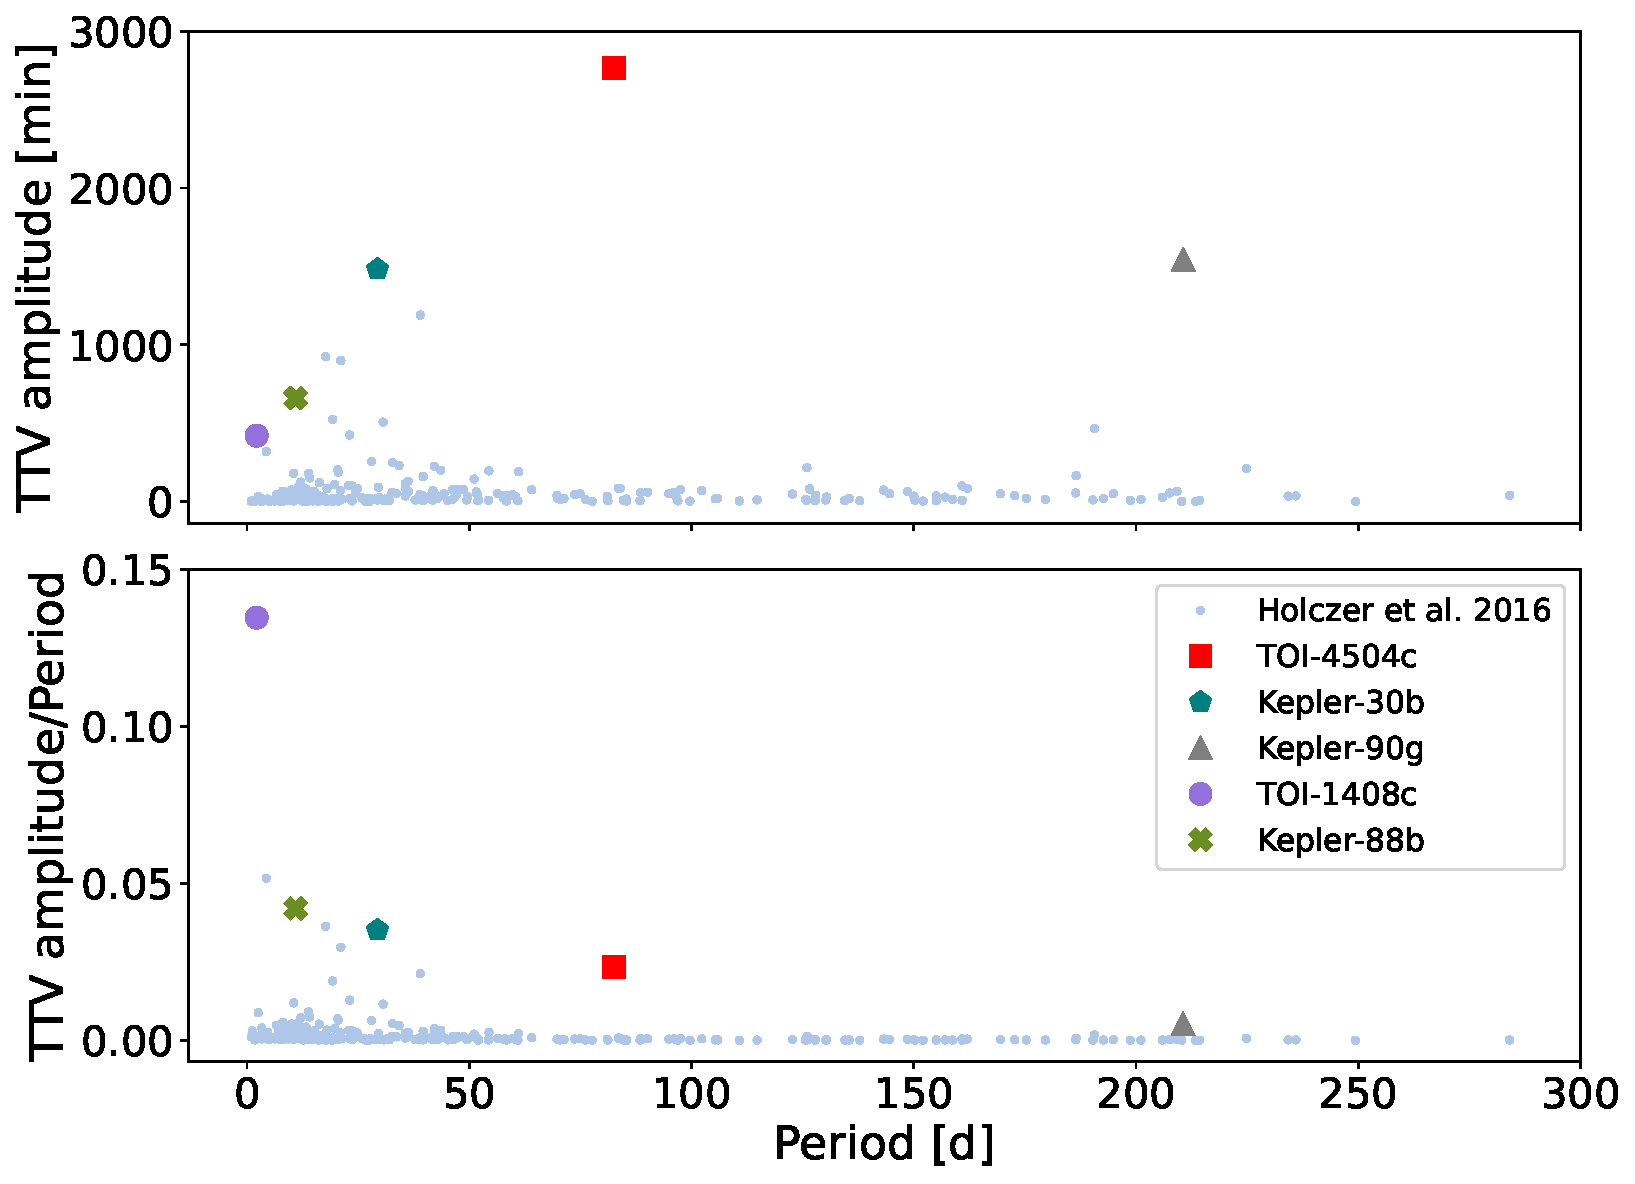
\includegraphics[width=0.48\textwidth]{holczer.pdf}
  \caption{Position of TOI-4504\,c, other planets with significant TTVs and planets from \cite{Holczer2016} in period-TTV amplitude and period-TTV amplitude and period ratio diagram. TTV amplitude is a peak-to-node amplitude of cosinus fit, for Kepler-90\,g it is the maximum observed difference between the time lapsed between consecutive transits.}
  \label{holczer}
\end{figure}


\cite{Holczer2016} made a transit timing catalogue of Kepler Objects of Interest (KOIs) and sorted out several KOIs that showed significant TTVs with long-term variations (see Table 5 in \cite{Holczer2016}. \autoref{holczer} shows TOI-4504\,c in context with other planets with significant TTVs. As can be seen from the top panel of \autoref{holczer}, the peak-to-node amplitude of TTVs of TOI-4504\,c is about twice as big as of Kepler-30\,b, a planet with the largest previously known TTV semi-amplitude \citep{Kepler30b}. However, when calculating the relative amplitude of the TTV with respect to the orbital period of the planet, TOI-4504\,c is not the record holder, although it still belongs to a small group of planets with large relative TTVs (the bottom panel of \autoref{holczer}).

The planet with the largest known TTVs relative to its orbital period is TOI-1408\,c, a sub-Neptune on a very short orbital period \citep{toi-1408}. Our dynamical solution implies that an observer located such that planet d was observed to transit (which is more than 1.6 times as likely as our view of planet c transiting) would observe TTVs more than 50\% larger than those that TESS observed for planet c. Thus, the ratio of d's TTVs to its orbital period would be almost as large as those of hot sub-Neptune TOI-1408 c \citep{toi-1408}.


%(SOMETHING TO BE SAID ABOUT TOI-1408 
%https://arxiv.org/pdf/2407.17798, which claims the largest TTV amplitude with respect to the orbital period. Michaela, please check where TOI4504 is in this context!).

Additional observations are needed to explain the large RV jitter observed in TOI-4504 and refine the orbital and physical parameters of the system. 
Although our fit to the TTVs is very good, additional observations are needed to further refine the orbital architecture of the TOI-4504\,c and d pair. Transits of TOI-4504\,c Nr. 29 and 31 (\autoref{Tab:TransitsPrediction}) will be observed by TESS in sectors 89 and 95, respectively. Due to significant uncertainties in the predicted transits, ground-based observations will be difficult. Observing campaigns on the nights around the predicted transits would be appreciated. TOI-4504 is within the southern PLATO field and should be monitored continuously for 2 years beginning in 2027 (transits 38 and further).
%While our TTV model component is nearly perfect, the RV model component was unable to fully resolve the large RV scatter around the fit, and the scatter noise remains unexplained. 

Since our RV model could not fully resolve the large RV scatter around the fit, the source of the RV jitter remains unclear. The current RV data conclusively confirm the presence of two resonant planets. However, more precise RV measurements are needed to determine the mass of the innermost planet, further constrain their orbital parameters and eccentricities of TOI-4504\,d and TOI-4504\,c, and eventually reveal the presence of additional planets in the system.

Since TOI-4504 is a rather faint target for the 2.2-m telescope with FEROS at La Silla, more precise RVs are urgently needed with facilities like ESPRESSO \citep{Pepe2021} to measure the planetary masses and eccentricities more accurately. We plan to continue our monitoring of TOI-4504 with transit and RV measurements, which will allow us to extend our orbital analysis, capturing the gravitational effects of the planets across the full transit light curve using a photo-dynamical model. These models can measure transit depths and durations, thereby better constraining the dynamic state of the system and shedding more light on the system's origin and migration processes.




%% IMPORTANT! The old "\acknowledgment" command has be depreciated. It was
%% not robust enough to handle our new dual anonymous review requirements and
%% thus been replaced with the acknowledgment environment. If you try to 
%% compile with \acknowledgment you will get an error print to the screen
%% and in the compiled pdf.
%% 
%% Also note that the akcnowlodgment environment does not support long amounts of text. If you have a lot of people and institutions to acknowledge, do not use this command. Instead, create a new \section{Acknowledgments}.

\section{Acknowledgments}
%\begin{acknowledgments}
We thank the anonymous referee for his/her comments that helped to improve the manuscript. M.V., M.S., and P.K. acknowledge support by Inter-transfer grant no LTT-20015. M.V. also acknowledges travel subsidy from grants ANID-23-05 and EU MSCA EXOWORLD project ID:101086149.
R.B. acknowledges support from FONDECYT Project 1241963 and from ANID -- Millennium  Science  Initiative -- ICN12\_009.
T.T. acknowledges support by the BNSF program "VIHREN-2021" project No. KP-06-DV/5.
M. T. P. acknowledges the support of Fondecyt-ANID fellowship no. 3210253 and ANID ASTRON-0037 project.
A.J.\ acknowledges support from ANID -- Millennium  Science  Initiative -- ICN12\_009 and AIM23-0001 and FONDECYT project 1210718.
K. A. C. acknowledges support from the TESS mission via subaward s3449 from MIT.
This work was funded by the Data Observatory Foundation.
This work was funded by ANID Vinculación Internacional FOVI220091.
This research has made use of the Exoplanet Follow-up Observation Program (ExoFOP; DOI: 10.26134/ExoFOP5) website, which is operated by the California Institute of Technology, under contract with the National Aeronautics and Space Administration under the Exoplanet Exploration Program.
Funding for the TESS mission is provided by NASA's Science Mission Directorate. We acknowledge the use of public TESS data from pipelines at the TESS Science Office and at the TESS Science Processing Operations Center. This paper includes data collected by the TESS mission that are publicly available from the Mikulski Archive for Space Telescopes (MAST). The specific observations analyzed can be accessed via \dataset[https://doi.org/10.17909/g52w-sk09]{https://doi.org/10.17909/g52w-sk09}. STScI is operated by the Association of Universities for Research in Astronomy, Inc., under NASA contract NAS5–26555. Support to MAST for these data is provided by the NASA Office of Space Science via grant NAG5–7584 and by other grants and contracts.
The results reported herein benefitted from collaborations and/or information exchange within NASA's Nexus for Exoplanet System Science (NExSS) research coordination network sponsored by NASA's Science Mission Directorate under Agreement No. 80NSSC21K0593 for the program "Alien Earths".
Resources supporting this work were provided by the NASA High-End Computing (HEC) Program through the NASA Advanced Supercomputing (NAS) Division at Ames Research Center for the production of the SPOC data products.
%\end{acknowledgments}

%% To help institutions obtain information on the effectiveness of their 
%% telescopes the AAS Journals has created a group of keywords for telescope 
%% facilities.
%
%% Following the acknowledgments section, use the following syntax and the
%% \facility{} or \facilities{} macros to list the keywords of facilities used 
%% in the research for the paper.  Each keyword is check against the master 
%% list during copy editing.  Individual instruments can be provided in 
%% parentheses, after the keyword, but they are not verified.

\vspace{5mm}
\facilities{TESS, MPG-2.2m/FEROS}

%% Similar to \facility{}, there is the optional \software command to allow 
%% authors a place to specify which programs were used during the creation of 
%% the manuscript. Authors should list each code and include either a
%% citation or url to the code inside ()s when available.

\software{{\textsc Exo-Striker} \citep{exostriker}, {\textsc juliet} \citep{juliet}, {\textsc ceres} \citep{ceres}, {\textsc zaspe} \citep{zaspe}, {\textsc tesseract} (Rojas, in prep.), {\textsc TESSCut} \citep{tesscut}, {\textsc lightkurve} \citep{lightkurve}, {\textsc dynesty} \citep{dynesty},
{\textsc batman} \citep{batman}, {\textsc celerite} \citep{celerite}}

%% Appendix material should be preceded with a single \appendix command.
%% There should be a \section command for each appendix. Mark appendix
%% subsections with the same markup you use in the main body of the paper.

%% Each Appendix (indicated with \section) will be lettered A, B, C, etc.
%% The equation counter will reset when it encounters the \appendix
%% command and will number appendix equations (A1), (A2), etc. The
%% Figure and Table counter will not reset.

%--------------------------------------------------------------------------------------------

\appendix

\setcounter{table}{0}
\renewcommand{\thetable}{A\arabic{table}}

\setcounter{figure}{0}
\renewcommand{\thefigure}{A\arabic{figure}}




%In this Appendix, we show in \autoref{sec:prediction} we list the estimated mid-transit time estimates of TOI-4504\,c,  in \autoref{} we list the estimated posterior probability distribution of our joint Doppler and TTV modeling with {\tt Exo-Striker}, in \autoref{}.....
 

%\section{TOI-4504 b}
%\label{Sec:TOI-4504bApendix}


\begin{table*}[ht]
% \begin{adjustwidth}{-4.0cm}{}
% \resizebox{0.69\textheight}{!}
% {\begin{minipage}{1.1\textwidth}

\centering
\caption{{Priors for the global Nested Sampling run, which aimed to identify the parameter space of TOI-4504\,d consistent with the TTVs of TOI4504\,c and RVs of TOI-4504.}}
\label{globalNS}

\begin{tabular}{lrrrrrrrr}     % 2 columns

\hline\hline  \noalign{\vskip 0.7mm}
Parameter \hspace{0.0 mm}& Planet d & Planet c \\
\hline \noalign{\vskip 0.7mm}

    $K$ [m\,s$^{-1}$]             & $\mathcal{U}$(     30.0,    120.0)& $\mathcal{U}$(    100.0,    250.0)\\
    $P$ [day]                     & $\mathcal{U}$(     20.0,     60.0) \& $\mathcal{U}$( 120.0,     300.0)& $\mathcal{U}$(     81.0,     83.0)\\
    $e\sin(\omega)$               & $\mathcal{U}$(     -0.10,      0.10)& $\mathcal{U}$(     -0.10,      0.10)\\
    $e\cos(\omega)$               & $\mathcal{U}$(     -0.10,      0.10)& $\mathcal{U}$(     -0.10,      0.10)\\
    $\lambda$ [deg]               & $\mathcal{U}$(   -180.0,    360.0)& $\mathcal{U}$(     70.0,    110.0)\\
    $i$ [deg]                     & $\mathcal{N}$(      86.0,    3.0)& $\mathcal{U}$(      89.7,    0.1)\\
    $\Omega$ [deg]                & 0 (fixed) & $\mathcal{N}$(      0.0,    30.0)\\

    RV off.$_{\rm FEROS}$  [m\,s$^{-1}$]& $\mathcal{U}$(   1950.0,   2150.0)\\
    RV jit.$_{\rm FEROS}$  [m\,s$^{-1}$]& $\mathcal{U}$(      0.0,    150.0)\\
    \\
\hline \noalign{\vskip 0.7mm}
    
\end{tabular}

% \end{minipage}}
% \end{adjustwidth}

%\tablefoot{\small }

\end{table*}

\section{Upcoming transits of TOI-4504 c}
\label{sec:prediction}
The N-body simulation, together with the best-fit solution of TTVs+RV analysis, allowed us to predict future transit times of TOI-4504\,c more than 10 years in advance \autoref{Tab:TransitsPrediction}. For completeness, we give also past transits since $t_{0}$ in \autoref{Tab:TransitsPrediction}. 

\begin{table*}
%\begin{center}
\centering
\caption{Predicted mid-transit times for TOI-4504\,c.}
\label{Tab:TransitsPrediction}
\begin{tabular}{cc | cc | cc | cc}
\hline \hline
Nr. & BJD & Nr. & BJD & Nr. & BJD & Nr. & BJD \\ \hline
1  & 2458401.4086$_{-0.0005}^{+0.0004}$ & 21 & 2460059.6184$_{-0.4373}^{+0.3886}$ & 41 & 2461715.7660$_{-1.2393}^{+1.0841}$ & 61 & 2463371.0909$_{-0.9278}^{+0.7731}$ \\
2  & 2458483.2231$_{-0.0153}^{+0.0148}$ & 22 & 2460142.5931$_{-0.3086}^{+0.2823}$ & 42 & 2461799.5893$_{-1.2186}^{+1.0956}$ & 62 & 2463454.1663$_{-1.4180}^{+1.1786}$ \\
3  & 2458565.1073$_{-0.0265}^{+0.0261}$ & 23 & 2460224.9812$_{-0.1876}^{+0.1716}$ & 43 & 2461883.1822$_{-1.0472}^{+0.9626}$ & 63 & 2463537.7434$_{-1.7736}^{+1.5151}$ \\
4  & 2458647.3635$_{-0.0406}^{+0.0390}$ & 24 & 2460306.9802$_{-0.1171}^{+0.1116}$ & 44 & 2461966.2880$_{-0.7521}^{+0.6963}$ & 64 & 2463621.5822$_{-1.8876}^{+1.6493}$ \\
5  & 2458730.2564$_{-0.0845}^{+0.0804}$ & 25 & 2460388.8415$_{-0.1206}^{+0.1139}$ & 45 & 2462048.8016$_{-0.4377}^{+0.4084}$ & 65 & 2463705.3773$_{-1.7615}^{+1.5622}$ \\
6  & 2458813.7926$_{-0.1493}^{+0.1328}$ & 26 & 2460470.8214$_{-0.2082}^{+0.1758}$ & 46 & 2462130.8606$_{-0.2422}^{+0.2417}$ & 66 & 2463788.8495$_{-1.4355}^{+1.3020}$ \\
7  & 2458897.6602$_{-0.1985}^{+0.1770}$ & 27 & 2460553.1805$_{-0.3916}^{+0.3396}$ & 47 & 2462212.7309$_{-0.2153}^{+0.1999}$ & 67 & 2463871.8038$_{-0.9814}^{+0.9202}$ \\
8  & 2458981.5652$_{-0.2339}^{+0.2063}$ & 28 & 2460636.1081$_{-0.6330}^{+0.5527}$ & 48 & 2462294.6947$_{-0.3225}^{+0.2820}$ & 68 & 2463954.2377$_{-0.6102}^{+0.5587}$ \\
9  & 2459065.2622$_{-0.2350}^{+0.2083}$ & 29 & 2460719.5920$_{-0.8437}^{+0.7512}$ & 49 & 2462377.0283$_{-0.5883}^{+0.5114}$ & 69 & 2464036.3360$_{-0.4052}^{+0.3851}$ \\
10 & 2459148.4917$_{-0.1932}^{+0.1722}$ & 30 & 2460803.4249$_{-0.9630}^{+0.8599}$ & 50 & 2462459.9463$_{-0.9861}^{+0.8540}$ & 70 & 2464118.3598$_{-0.4653}^{+0.3946}$ \\
11 & 2459231.1206$_{-0.1300}^{+0.1187}$ & 31 & 2460887.3192$_{-0.9664}^{+0.8721}$ & 51 & 2462543.4456$_{-1.3014}^{+1.1507}$ & 71 & 2464200.5739$_{-0.7364}^{+0.5998}$ \\
12 & 2459313.2552$_{-0.0768}^{+0.0690}$ & 32 & 2460970.9786$_{-0.8496}^{+0.7765}$ & 52 & 2462627.2792$_{-1.4381}^{+1.2986}$ & 72 & 2464283.1879$_{-1.2111}^{+1.0083}$ \\
13 & 2459395.1287$_{-0.0530}^{+0.0510}$ & 33 & 2461054.1342$_{-0.6253}^{+0.5618}$ & 53 & 2462711.1361$_{-1.4059}^{+1.2869}$ & 73 & 2464366.2819$_{-1.7046}^{+1.4592}$ \\
14 & 2459476.9771$_{-0.0608}^{+0.0582}$ & 34 & 2461136.6787$_{-0.3664}^{+0.3407}$ & 54 & 2462794.7524$_{-1.2161}^{+1.1275}$ & 74 & 2464449.7853$_{-2.1040}^{+1.8135}$ \\
15 & 2459559.0306$_{-0.1041}^{+0.0975}$ & 35 & 2461218.7611$_{-0.2035}^{+0.2007}$ & 55 & 2462877.9109$_{-0.8877}^{+0.8377}$ & 75 & 2464533.5273$_{-2.2332}^{+2.0046}$ \\
16 & 2459641.5272$_{-0.1941}^{+0.1779}$ & 36 & 2461300.6731$_{-0.1945}^{+0.1820}$ & 56 & 2462960.5230$_{-0.5423}^{+0.5304}$ & 76 & 2464617.2672$_{-2.1452}^{+1.9669}$ \\
17 & 2459724.6306$_{-0.3385}^{+0.2897}$ & 37 & 2461382.7407$_{-0.3265}^{+0.2812}$ & 57 & 2463042.6845$_{-0.3300}^{+0.3270}$ & 77 & 2464700.7314$_{-1.7739}^{+1.6552}$ \\
18 & 2459808.2733$_{-0.4565}^{+0.3962}$ & 38 & 2461465.2669$_{-0.6066}^{+0.5158}$ & 58 & 2463124.5967$_{-0.2574}^{+0.2358}$ & 78 & 2464783.7092$_{-1.2096}^{+1.1508}$ \\
19 & 2459892.1846$_{-0.5243}^{+0.4561}$ & 39 & 2461548.3851$_{-0.9165}^{+0.7916}$ & 59 & 2463206.4837$_{-0.3098}^{+0.2714}$ & 79 & 2464866.1730$_{-0.7025}^{+0.6756}$ \\
20 & 2459976.0671$_{-0.5178}^{+0.4589}$ & 40 & 2461631.9600$_{-1.1403}^{+0.9770}$ & 60 & 2463288.5747$_{-0.5271}^{+0.4398}$ & 80 & 2464948.2903$_{-0.4299}^{+0.4509}$\\ \hline \hline
\end{tabular}
\tablecomments{Nr gives the number of the transit since t$_0$, and BJD gives the mid-transit times.}
%\end{center}
\end{table*}



%\section{Activity indicators and radial velocity data}

\begin{table*}
\begin{rotatetable*}
\begin{center}
%\centering
\caption{Radial velocity and activity indices of TOI-4504 measured with FEROS.}
\label{RV_feros}
\scalebox{0.9}{
\begin{tabular}{ccccccccc}

\hline \hline
BJD             & RV [m/s]           & Bisector     & FWHM    & SNR & $\rm{H}_{\alpha}$      & $\log(\rm{R_{HK}})$  & Na\,II             & He\,I                            \\ \hline 
2458912.730428  & $2023.5 \pm 10.1$ & $-48 \pm 15 $ & 9.9507  & 49     & $0.1554 \pm 0.004  $& $-4.4426 \pm 0.0641 $&$ 0.2966 \pm 0.0073 $&$ 0.5121 \pm 0.0097 $\\
2458917.7301462 & $1774.9 \pm 11.7$ & $-39 \pm 17 $ & 9.9237  & 41     & $0.1346 \pm 0.0043 $& $-5.4889 \pm 0.6482 $&$ 0.3188 \pm 0.0086 $&$ 0.5219 \pm 0.011  $\\
2458925.5538544 & $1992.5 \pm 26.5$ & $75 \pm 34  $ & 10.0707 & 17     & $0.2872 \pm 0.023  $& $-4.1016 \pm 0.0692 $&$ 0.5544 \pm 0.0441 $&$ 0.6636 \pm 0.0436 $\\
2458925.5970903 & $1869.9 \pm 11.3$ & $-66 \pm 16 $ & 9.9409  & 42     & $0.1503 \pm 0.0045 $& $-4.9067 \pm 0.1358 $&$ 0.2471 \pm 0.0076 $&$ 0.536 \pm 0.0106  $\\
2459189.7431016 & $2247.1 \pm 10$   & $-46 \pm 15 $ & 9.8113  & 47     & $0.1494 \pm 0.0042 $& $-5.2786 \pm 0.1929 $&$ 0.2439 \pm 0.0069 $&$ 0.5176 \pm 0.01   $\\
2459192.7143168 & $2255.4 \pm 14.5$ & $-79 \pm 20 $ & 9.7936  & 32     & $0.1557 \pm 0.0073 $& $-4.706 \pm 0.1078  $&$ 0.2373 \pm 0.0124 $&$ 0.4613 \pm 0.0152 $\\
2459207.7670343 & $2210.2 \pm 10.6$ & $-4 \pm 15  $ & 9.8256  & 45     & $0.1463 \pm 0.0043 $& $-5.0808 \pm 0.1269 $&$ 0.1944 \pm 0.0069 $&$ 0.5163 \pm 0.0102 $\\
2459211.7211734 & $2228.6 \pm 10.9$ & $21 \pm 16  $ & 9.8664  & 44     & $0.1596 \pm 0.0047 $& $-5.0505 \pm 0.1226 $&$ 0.2142 \pm 0.0073 $&$ 0.5216 \pm 0.0104 $\\
2459218.7262622 & $2038.1 \pm 10$   & $-47 \pm 15 $ & 9.8061  & 49     & $0.1296 \pm 0.0036 $& $-4.9215 \pm 0.1023 $&$ 0.2176 \pm 0.0061 $&$ 0.5052 \pm 0.0088 $\\
2459260.6382415 & $1877.8 \pm 12$   & $-14 \pm 17 $ & 9.8243  & 39     & $0.1857 \pm 0.0058 $& $-5.2035 \pm 0.2064 $&$ 0.2347 \pm 0.0086 $&$ 0.513 \pm 0.0116  $\\
2459272.776905  & $2081.6 \pm 13.4$ & $4 \pm 19   $ & 9.8138  & 35     & $0.1369 \pm 0.0055 $& $-4.5168 \pm 0.0767 $&$ 0.2836 \pm 0.0105 $&$ 0.5342 \pm 0.0138 $\\
2459274.716173  & $2224.5 \pm 10.6$ & $-1 \pm 15  $ & 9.7323  & 45     & $0.1372 \pm 0.0042 $& $-5.4107 \pm 0.3654 $&$ 0.266 \pm 0.0074  $&$ 0.5071 \pm 0.0097 $\\
2459276.7156498 & $2134.9 \pm 12.9$ & $-46 \pm 18 $ & 10.0024 & 36     & $0.1444 \pm 0.0048 $& $-999 \pm -999      $&$ 0.2532 \pm 0.0087 $&$ 0.5305 \pm 0.0119 $\\
2459282.5358342 & $2267.5 \pm 10.6$ & $11 \pm 15  $ & 9.8555  & 45     & $0.1412 \pm 0.0041 $& $-5.1246 \pm 0.145  $&$ 0.2665 \pm 0.0074 $&$ 0.5166 \pm 0.0103 $\\
2459539.7731663 & $2231.6 \pm 10.9$ & $48 \pm 16  $ & 10.0306 & 44     & $0.1836 \pm 0.0047 $& $-4.5648 \pm 0.0608 $&$ 0.1945 \pm 0.007  $&$ 0.5304 \pm 0.0105 $\\
2459545.7659941 & $2043.8 \pm 12.8$ & $-15 \pm 18 $ & 9.5975  & 36     & $0.238 \pm 0.0062  $& $-6.2329 \pm 3.4563 $&$ 0.2811 \pm 0.01   $&$ 0.5237 \pm 0.0123 $\\
2459590.7117932 & $1786 \pm 13.9$   & $41 \pm 19  $ & 9.807   & 33     & $0.2119 \pm 0.0067 $& $-4.6104 \pm 0.1074 $&$ 0.2212 \pm 0.0112 $&$ 0.5304 \pm 0.0152 $\\
2459644.7122898 & $2181.7 \pm 14.5$ & $-104 \pm 20$ & 9.5813  & 32     & $0.2234 \pm 0.0066 $& $-4.6445 \pm 0.2152 $&$ 0.3935 \pm 0.0129 $&$ 0.5021 \pm 0.0141 $\\
2459649.629842  & $2140.1 \pm 10$   & $-118 \pm 15 $& 9.8357  & 49     & $0.1979 \pm 0.0041 $& $-999 \pm -999      $&$ 0.2381 \pm 0.0065 $&$ 0.4922 \pm 0.0091 $\\
2459652.6796063 & $2016 \pm 12.1$   & $104 \pm 17  $& 9.7958  & 39     & $0.2288 \pm 0.0057 $& $-4.5995 \pm 0.0931 $&$ 0.3102 \pm 0.0094 $&$ 0.5146 \pm 0.0116 $\\
2459657.727332  & $1724.3 \pm 13$   & $-101 \pm 18$ & 10.1905 & 36     & $0.1698 \pm 0.005  $& $-999 \pm -999     $ &$ 0.3019 \pm 0.0097 $&$ 0.5582 \pm 0.0127 $\\
2459661.6841378 & $1910.5 \pm 16.9$ & $-109 \pm 18$& 10.0861 & 38     & $0.24 \pm 0.0062   $& $-999 \pm -999      $& $0.2641 \pm 0.0095 $& $0.538 \pm 0.0127  $\\
2459662.6697007 & $1817.8 \pm 15.2$ & $83 \pm 21  $ & 10.0149 & 30     & $0.2389 \pm 0.0064 $& $-999 \pm -999      $&$ 0.3149 \pm 0.0112 $&$ 0.5291 \pm 0.0141 $\\
2459685.5096644 & $2094.7 \pm 11.7$ & $-106 \pm 17$ & 9.8454  & 41     & $0.1575 \pm 0.0047 $& $-5.2897 \pm 0.36   $&$ 0.3526 \pm 0.0094 $&$ 0.5028 \pm 0.0106 $\\
2459687.5617665 & $2190.1 \pm 10.1$ & $-120 \pm 15$ & 10.0629 & 49     & $0.1979 \pm 0.0048 $& $-4.9255 \pm 0.1053 $&$ 0.3099 \pm 0.0079 $&$ 0.4911 \pm 0.0098 $\\
2459691.5839601 & $2311.2 \pm 14.5$ & $106 \pm 20 $ & 9.8589  & 32     & $0.2592 \pm 0.0073 $& $-4.8472 \pm 0.2618 $&$ 0.4324 \pm 0.0136 $&$ 0.4913 \pm 0.0144 $\\
2459704.623859  & $2092 \pm 15.2$   & $-148 \pm 21$ & 9.914   & 30     & $0.1667 \pm 0.0054 $& $-999 \pm -999      $&$ 0.5008 \pm 0.0121 $&$ 0.5023 \pm 0.0128 $\\
2460031.6812879 & $2174.8 \pm 11.7$ & $0 \pm 17   $ & 9.9468  & 41     & $0.2287 \pm 0.006  $& $-999 \pm -999      $&$ 0.2467 \pm 0.009  $&$ 0.5173 \pm 0.0123 $\\
2460035.6102046 & $2142.3 \pm 9.8$  & $-60 \pm 15 $ & 9.8799  & 50     & $0.1402 \pm 0.0047 $& $-4.7232 \pm 0.0919 $&$ 0.239 \pm 0.006   $&$ 0.5235 \pm 0.0088 $\\
2460047.6196292 & $2185.9 \pm 11.3$ & $-29 \pm 16 $ & 9.8589  & 42     & $0.1388 \pm 0.0075 $& $-6.2879 \pm 4.636  $&$ 0.2799 \pm 0.0081 $&$ 0.5235 \pm 0.0109 $\\
2460049.6297281 & $2235.2 \pm 11.7$ & $-11 \pm 17 $ & 9.9268  & 41     & $0.1787 \pm 0.0048 $& $-4.5127 \pm 0.133  $&$ 0.2593 \pm 0.0081 $&$ 0.5182 \pm 0.0105 $\\
2460053.5979115 & $2273 \pm 10.3$   & $-28 \pm 15 $ & 9.8936  & 47     & $0.1627 \pm 0.0042 $& $-4.6646 \pm 0.0912 $&$ 0.2688 \pm 0.0072 $&$ 0.4967 \pm 0.0094 $\\
2460064.5861888 & $2101.8 \pm 14$   & $-7 \pm 19  $ & 10.0588 & 33     & $0.215 \pm 0.0065  $& $-4.6949 \pm 0.1573 $&$ 0.3868 \pm 0.0117 $&$ 0.5458 \pm 0.0134 $\\
2460067.4999667 & $1900.5 \pm 12.5$ & $12 \pm 18  $ & 10.1785 & 38     & $0.1855 \pm 0.0056 $& $-4.7865 \pm 0.1005 $&$ 0.475 \pm 0.0112  $&$ 0.54 \pm 0.0121  $ \\
2460100.5511551 & $1911 \pm 14.1$   & $-213 \pm 18$ & 10.2172 & 36     & $0.198 \pm 0.0073 $ & $-4.0598 \pm 0.0348 $&$ 0.3902 \pm 0.0125 $&$ 0.4311 \pm 0.0126$ \\ 
2460404.6178393 & $1978.3 \pm 10.4$ & $-60 \pm 15$  & 9.9642 & 47 & $0.1620 \pm 0.0044$ &  $-5.0872 \pm 0.2347$ & $0.3396 \pm 0.0081$ & $0.5046 \pm 0.0100$\\
2460407.5764817 & $1909 \pm 11$     & $68 \pm 16$   & 9.8798 & 44 & $0.1485 \pm 0.0044$ & $-5.1868 \pm 0.2541$ & $0.3106 \pm 0.0082$ & $0.5284 \pm 0.0108$\\
2460411.5489370 & $1878.9 \pm 12.9$ & $90 \pm 18$   & 9.9523 & 36 & $0.1684 \pm 0.0054$ & $-5.0893 \pm 0.2633$ & $0.4273 \pm 0.0109$ & $0.4882 \pm 0.0116$\\
2460433.5833358 & $2270.6 \pm 20.6$ & $-159 \pm 28$ & 9.6584 & 21 & $0.3803 \pm 0.0149$ & $-3.9235 \pm 0.0538$ & $2.5052 \pm 0.0535$ & $0.5286 \pm 0.0315$\\
\hline \hline
\end{tabular}}
\end{center}
\end{rotatetable*}
\end{table*}

\begin{figure*}
    
    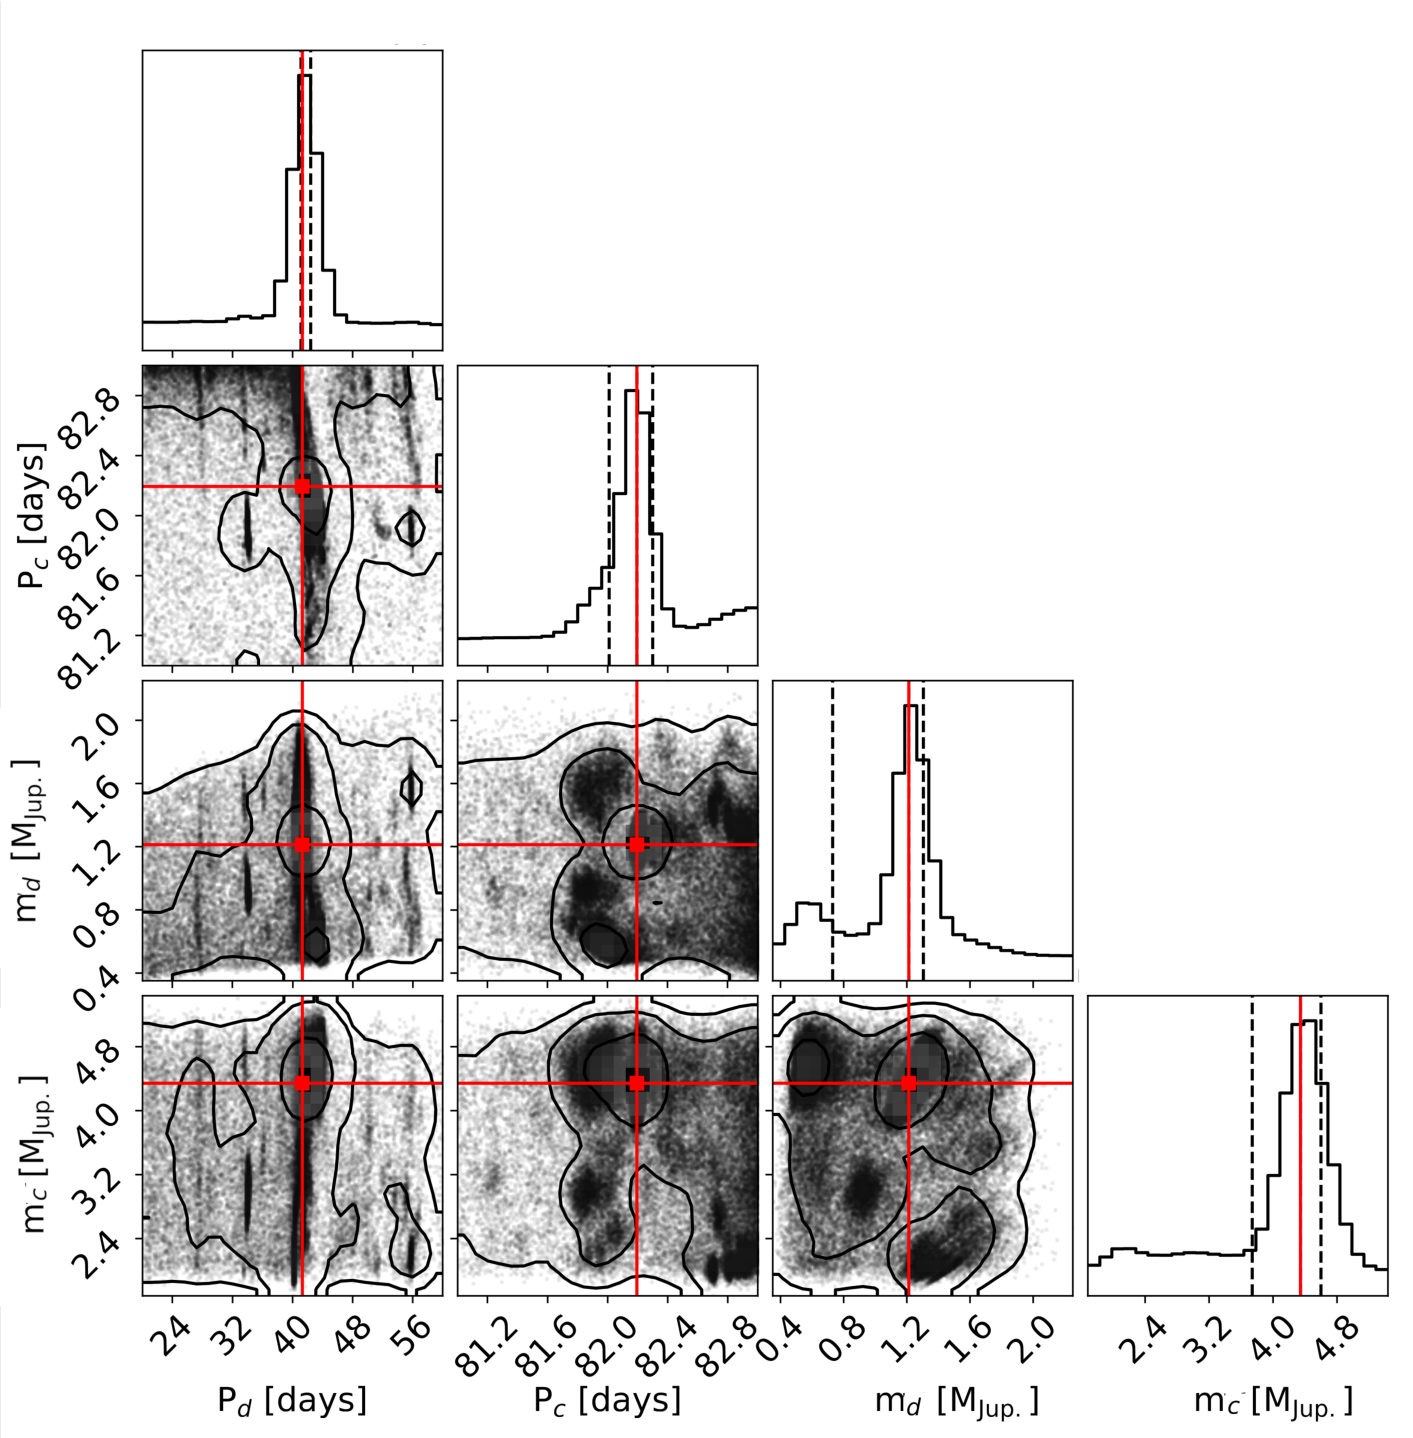
\includegraphics[width=17cm]{2pl_TTV+RVs_Ns_Large_priors_P_m.pdf}
    \caption{Posterior distribution from a global joint TTV+RV static nested sampling search with very large priors, which aim to map the possible periods for the non-transiting perturber TOI-4504\,d. The posterior is multi-modal implying that different period ratios could produce the observed TTVs, but the 41-day period massive planet leads to significantly better fits pointing towards a 2:1 period ratio commensurability with TOI-4504\,c}
    \label{Nest_samp_ttv}
    
\end{figure*} 



\begin{figure*}
    
    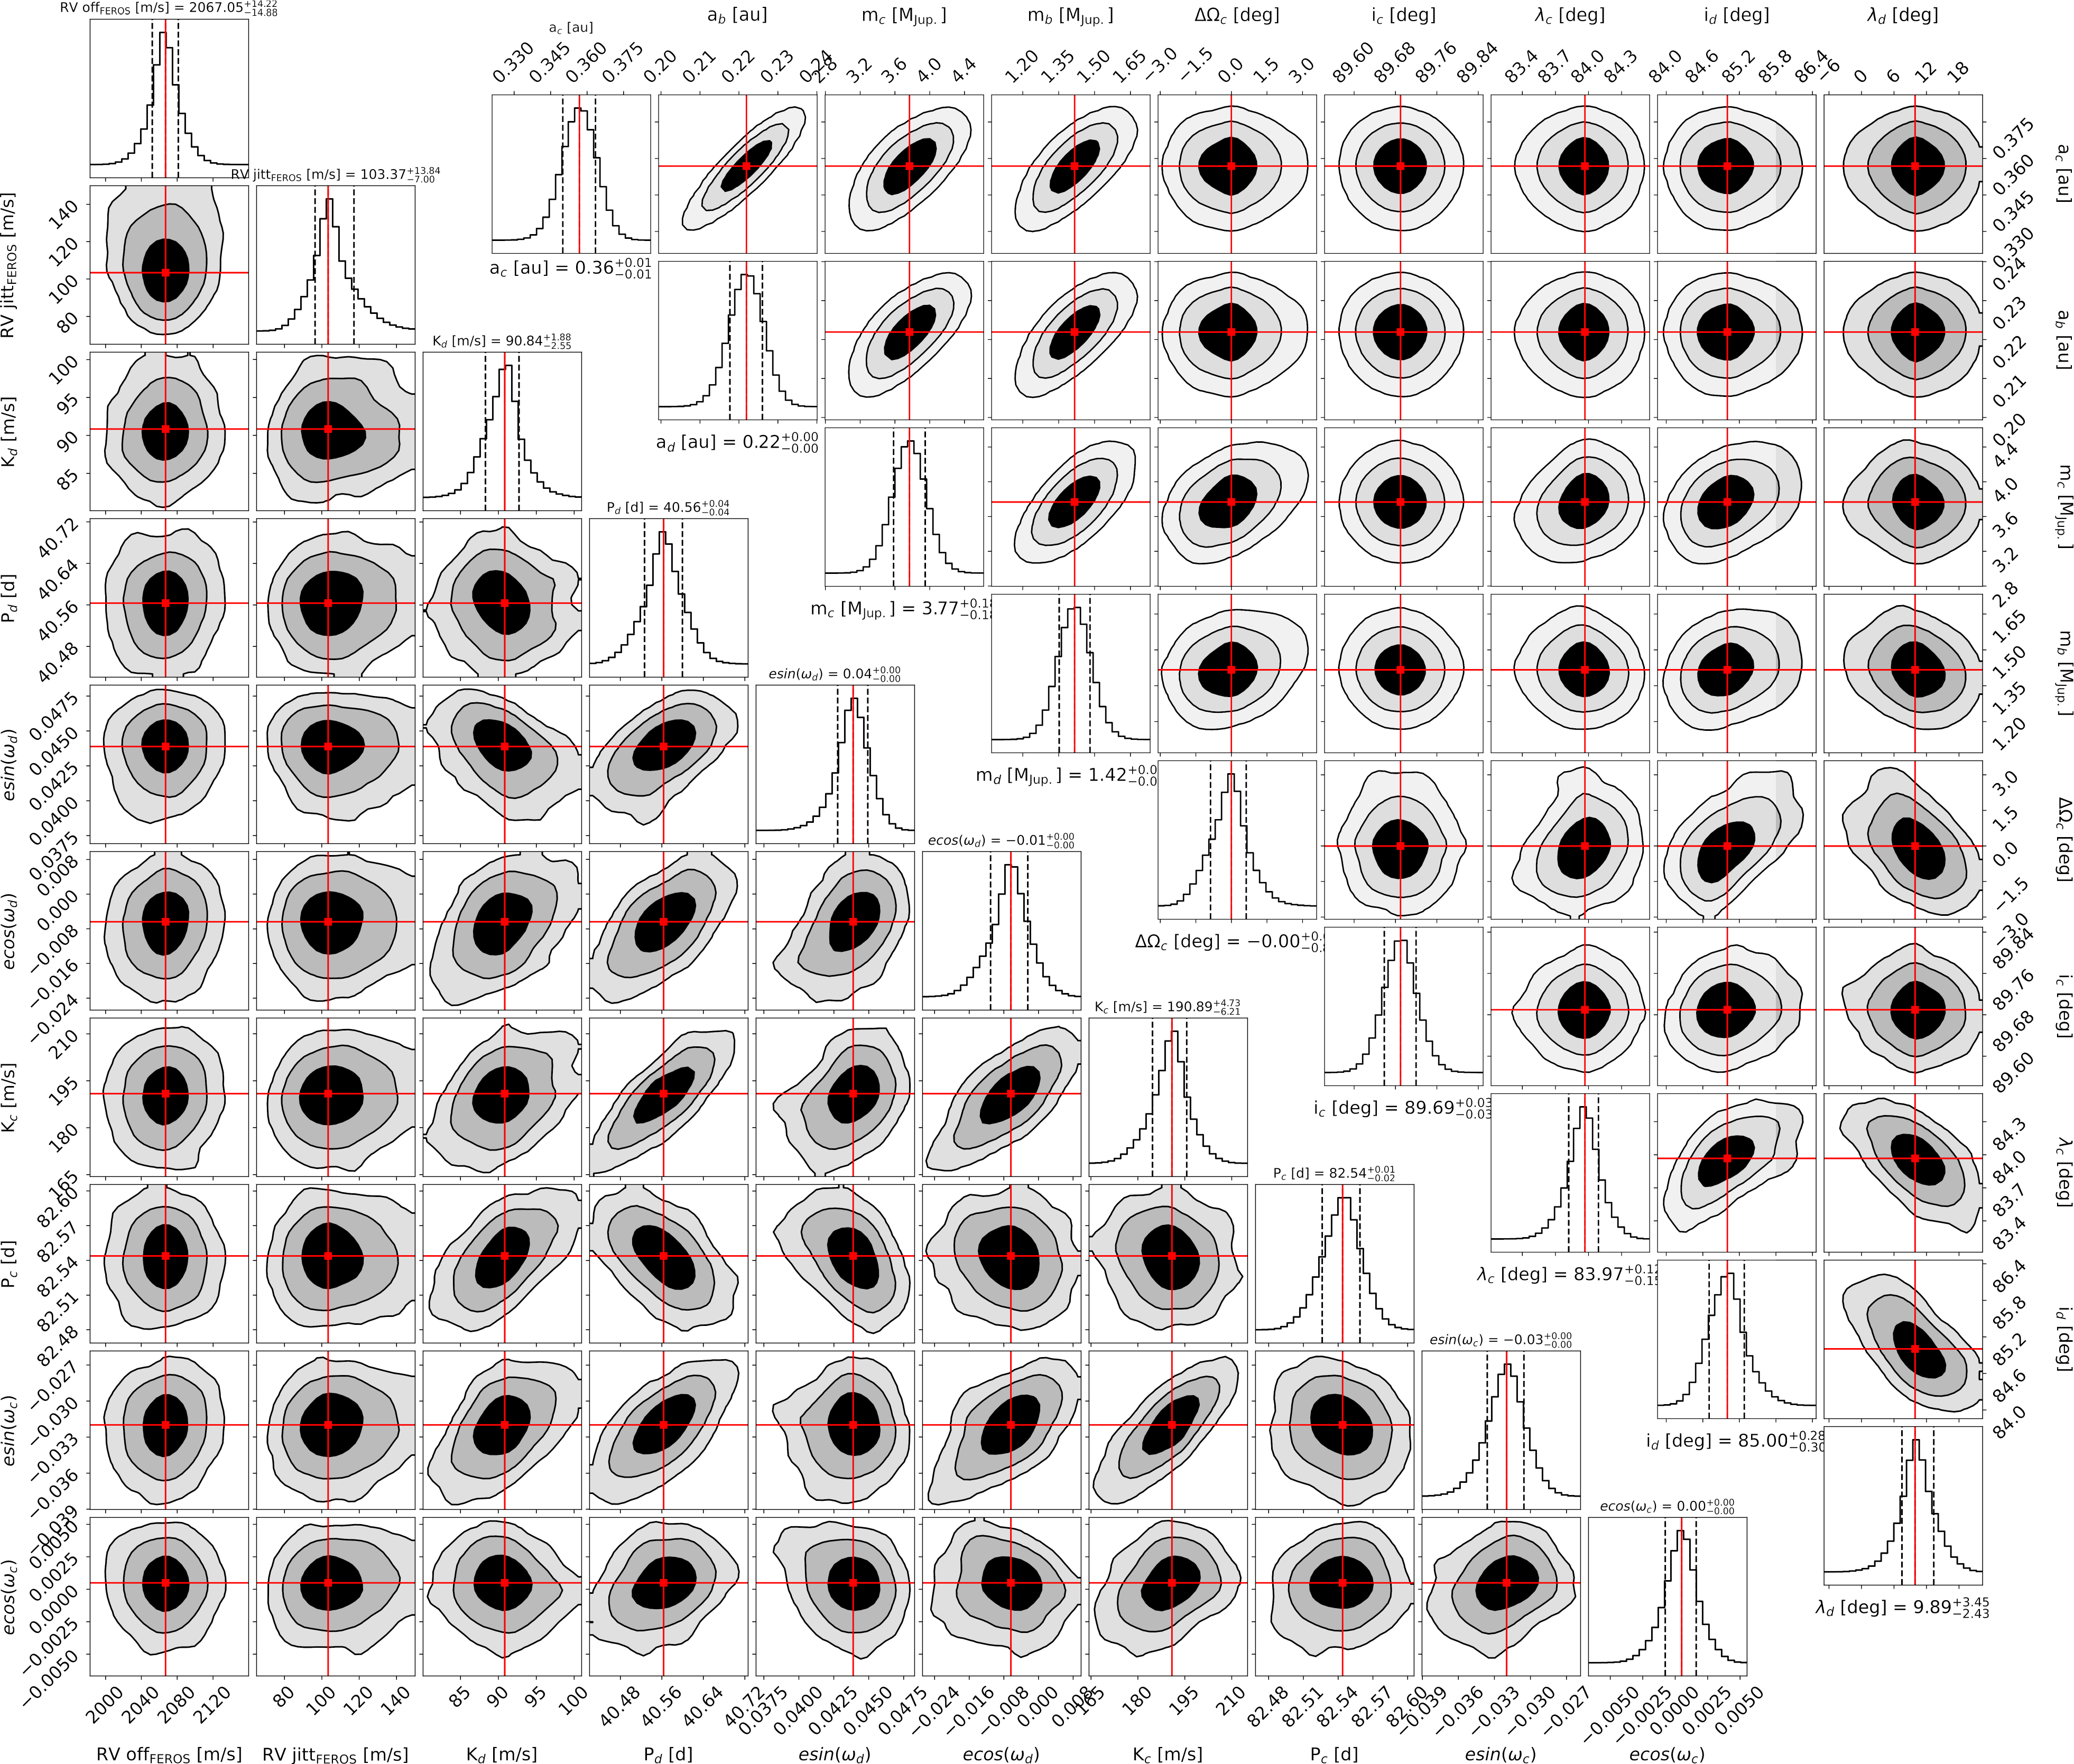
\includegraphics[width=17cm]{MCMC_posteriors.pdf}
    \caption{Posterior distribution from a focused joint TTV+RV MCMC sampling, whose results are listed in \autoref{NS_params}. The median values of the fitted and derived posteriors are marked in red. The black contour lines represent the 1,\,2 and 3$\sigma$ intervals of the distribution.}
    
    \label{mcmc_posteriors}
    
\end{figure*} 

%\section{Orbital modeling of the TOI-4504 b \& c based on TTV and RV data}


% \end{table}
%% For this sample we use BibTeX plus aasjournals.bst to generate the
%% the bibliography. The sample631.bib file was populated from ADS. To
%% get the citations to show in the compiled file do the following:
%%
%% pdflatex sample631.tex
%% bibtext sample631
%% pdflatex sample631.tex
%% pdflatex sample631.tex

\bibliography{sample631}{}
\bibliographystyle{aasjournal}

%% This command is needed to show the entire author+affiliation list when
%% the collaboration and author truncation commands are used.  It has to
%% go at the end of the manuscript.
%\allauthors

%% Include this line if you are using the \added, \replaced, \deleted
%% commands to see a summary list of all changes at the end of the article.
%\listofchanges

\end{document}

% End of file `sample631.tex'.
